\documentclass[xcolor={usenames,svgnames}]{beamer}
%%%%%%%%%%%%%%%%%%%
% Now set the style TODO: change this!!
%%%%%%%%%%%%%%%%%%%
\usetheme{Madrid}
\usecolortheme{dolphin}
% \setbeamertemplate{page number in head/foot}{}
% Get rid of navigation symbols
\setbeamertemplate{navigation symbols}{}
%%%%%%%%%%%%%%%%%
% custom headline
%%%%%%%%%%%%%%%%%
\setbeamertemplate{headline}{%
\leavevmode%
  \hbox{%
    \begin{beamercolorbox}[wd=0.5\paperwidth,ht=2.5ex,dp=1.125ex]{palette tertiary}%
    \hskip0pt plus1filll \insertsubsection \hspace{2pt}
    \end{beamercolorbox}%
    \begin{beamercolorbox}[wd=0.5\paperwidth,ht=2.5ex,dp=1.125ex]{palette secondary}%
    \hskip 2pt \insertsection
    \end{beamercolorbox}%
  }
}
%%%%%%%%%%
% Packages
%%%%%%%%%%
\usepackage[utf8]{inputenc}
\usepackage{amssymb}
\usepackage{booktabs}
\usepackage{booktabs}
\usepackage{caption}
\usepackage{csquotes}
\usepackage{longtable}
\usepackage{pifont}
\usepackage{siunitx}
\usepackage{subcaption}
\usepackage{tcolorbox}
\usepackage{tabularx}
\usepackage[framemethod=TikZ]{mdframed}

% define beamer citation command
\newcommand{\beamercite}[2]{\href{#2}{{\color{ForestGreen}\fontsize{6}{7}\selectfont{[#1]}}}}
\newcommand{\genericauthor}{NNPDF \& N3PDF}

\DeclareCaptionFormat{smol}{ \tiny {\color{blue}Fig#2} #3}

%%%%%%%%%%
% metadata
%%%%%%%%%%
\author[NNPDF \& N3PDF]{
Christopher Schwan and
Rosalyn Pearson and
Felix Hekhorn and
Tommaso Giani and
Juan Cruz-Martinez and
Roy Stegeman and
Michael Wilson and
Zahari Kassabov and
Tanjona Rabemananjara
}
% for footer
\title{NNPDF}
\date{PDF4LHC}

\AtBeginSection[]{
  \author[\genericauthor]{} % revert to generic author between section
  \institute{} % and revert institute
  % remove custom buffer frame - use SF's
  %  \begin{frame}
  %  \vfill
  %  \centering
  %  \begin{beamercolorbox}[sep=8pt,center,shadow=true,rounded=true]{title}
  %    \usebeamerfont{title}\insertsectionhead\par
  %  \end{beamercolorbox}
  %  \vfill
  %  \end{frame}
}


\providecommand{\tightlist}{%
  \setlength{\itemsep}{0pt}\setlength{\parskip}{0pt}}

\begin{document}
\section{Theory Developments}
\title{NNPDF}
\author[Christopher Schwan]{}
\institute{Universit\`a di Milano}
\date{PDF4LHC}

\subsection{NLO EW corrections for PDF fits}

\begin{frame}{NLO EW corrections for PDF fits}
\begin{columns}[onlytextwidth]
\begin{column}{0.45\textwidth}

\begin{block}{What do we need?}
\begin{itemize}
\item[\ding{51}] At least QED corrections in DGLAP
\item[\ding{55}] NLO EW (including NLO QCD+EW) corrections for all PDF processes
\end{itemize}
\end{block}

\vspace*{0.7cm}

\begin{block}{Motivation?}
\begin{itemize}
\item In principle: always add EW corrections when we have them, more precision
\item In practice: cuts can be relaxed: DY large-mass region, \ldots
\item Requested at PDF4LHC for a long time
\end{itemize}
\end{block}
\end{column}
\begin{column}{0.45\textwidth}
\begin{block}{Problems to be solved}
\begin{itemize}
\item[\ding{51}] Need corrections in the form of \alert{interpolation grids}: PineAPPL, interfacing with Madgraph5\_aMC@NLO (see \href{https://arxiv.org/abs/2008.12789}{arXiv:2008.12789})
\item[\ding{51}] Careful selection of data: no subtraction of FSR, no photon-initiated subtraction, proper observable definition
\item[\ding{55}] Produce all predictions and implement all (changed) data (WIP)
\item[$\rightarrow$] Run fit
\end{itemize}
\end{block}
\end{column}
\end{columns}
\end{frame}

\begin{frame}{Example: Drell--Yan @ 14 TeV}
\begin{columns}[T,onlytextwidth]
\begin{column}{0.5\textwidth}
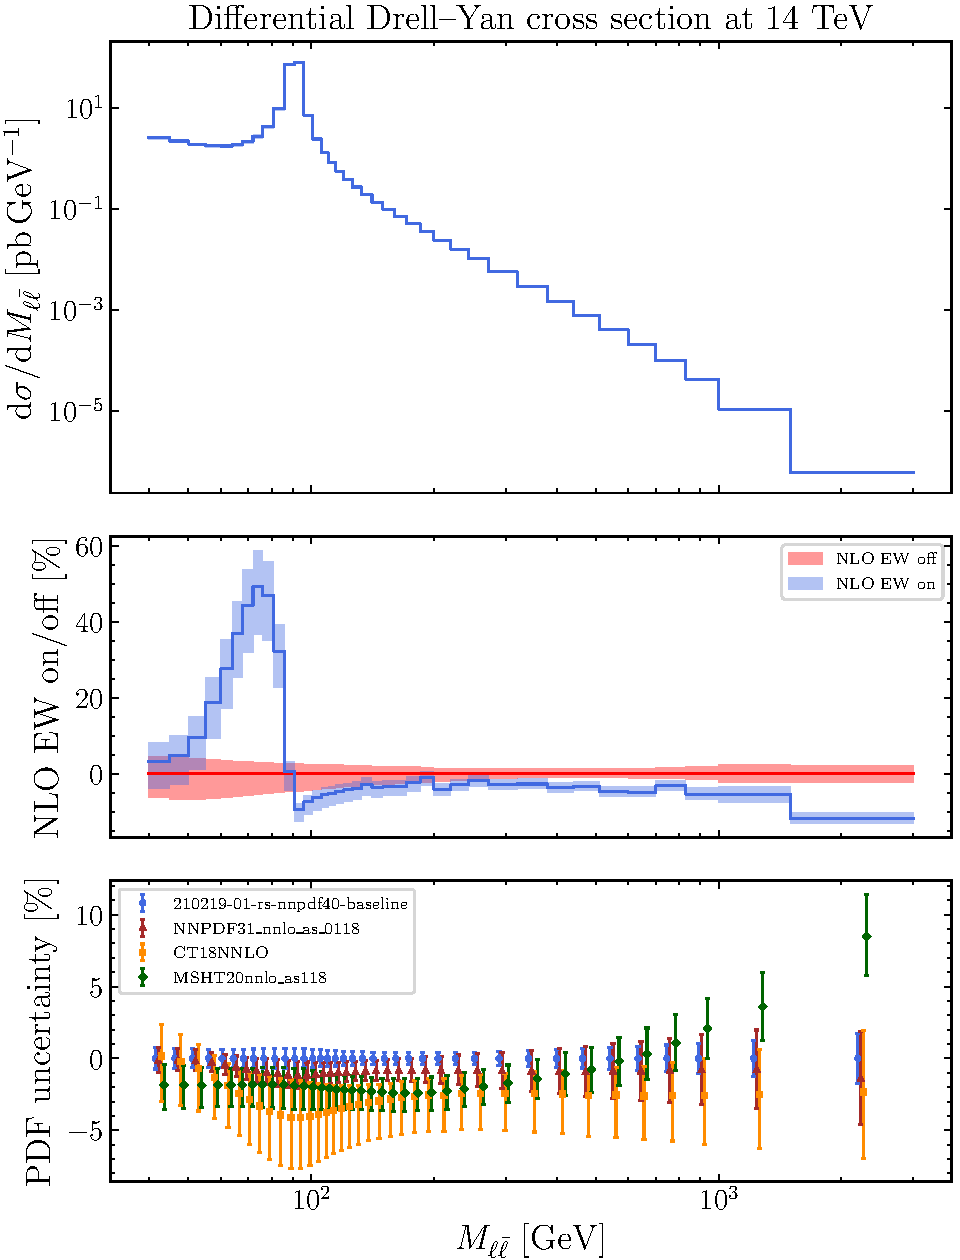
\includegraphics[height=.9\textheight]{ew_corrections/figures/NNPDF40_DY_Z}
\end{column}
\begin{column}{0.5\textwidth}
\begin{itemize}
\vspace*{0.1cm}
\item binning from CMS DY @ \SI{13}{\tera\electronvolt}: \href{https://arxiv.org/abs/1812.10529}{arXiv:1812.10529}
\vspace*{2.3cm}
\item FSR distort the Z peak, weak corrections in the large-mass region
\vspace*{1.3cm}
\item PDF uncertainties for NNPDF4.0, 3.1, CT18NNLO, and MSHT20
\end{itemize}
\end{column}
\end{columns}
\end{frame}

\author[Rosalyn Pearson]{}
\institute{University of Edinburgh}
\subsection{Nuclear and deuteron uncertainties}


\begin{frame}[fragile]{Deuteron and nuclear uncertainties}
We use an {\bf uncertainty} rather than a correcting the central value.
\newline
Theory covariance formalism previously developed in NNPDF.
      \begin{block}{Theory covariance matrix \tiny{ \textcolor{green}{[Ball, Nocera, Pearson: Eur.Phys.J.C 79 (2019) 3, 282 \& Eur.Phys.J.C 81 (2021) 1, 37]}}}
        \begin{equation}
            S_{ij} = \frac{1}{N_{rep}} \sum_k^{N_{rep}} \Delta_i^{(k)}\Delta_j^{(k)}
        \end{equation}
        \begin{equation}
            \Delta_i^{(k)} = T_i^{N}[f_{N}^{(k)}] - T_i^{N}[f_{p}]
        \end{equation}
      \end{block}
      
    \textbf{Deuteron:} NNLO deuteron PDFs fitted in NNPDF methodology 
    
    \textbf{Heavy nuclear:} NLO heavy nuclear PDFs from nNNPDF2.0 \tiny{ \textcolor{green}{[Abdul Khalek et al.: JHEP 09 (2020) 183]}}
  \begin{table}
    \caption{$\chi^2$ per deuteron/nuclear dataset}
        \resizebox{\linewidth}{!}{
    \begin{tabular}{rllllllll}
      \toprule
      Fit & {\bf Total} & BCDMS d & SLAC d & NMC p/d & E866/NuSea p/d & E605 Cu & NuTeV Fe & CHORUS Pb \\
      \midrule
      NNPDF4.0 & {\bf 1.174} & 1.015 & 0.4972 & 0.8194 & 0.3971 & 0.4907 & 0.4602 & 0.9372 \\
      No nuc unc & {\bf 1.265} & 1.313 & 0.8217 & 0.8167 & 0.8195 & 1.154 & 0.4569 & 1.165 \\
      \bottomrule
    \end{tabular}}
  \end{table}
\end{frame}

\begin{frame}{Per-point uncertainties}
\footnotesize{Deuteron (top) and heavy nuclear (bottom) }
\newline
\footnotesize{\textcolor{violet}{{\bf C:} experimental uncertainties}}
\newline
\footnotesize{\textcolor{orange}{{\bf S:} theory uncertainties (nuclear)}}
\newline
\footnotesize{\textcolor{cyan}{{\bf C+S:} total}}
  \begin{figure}
    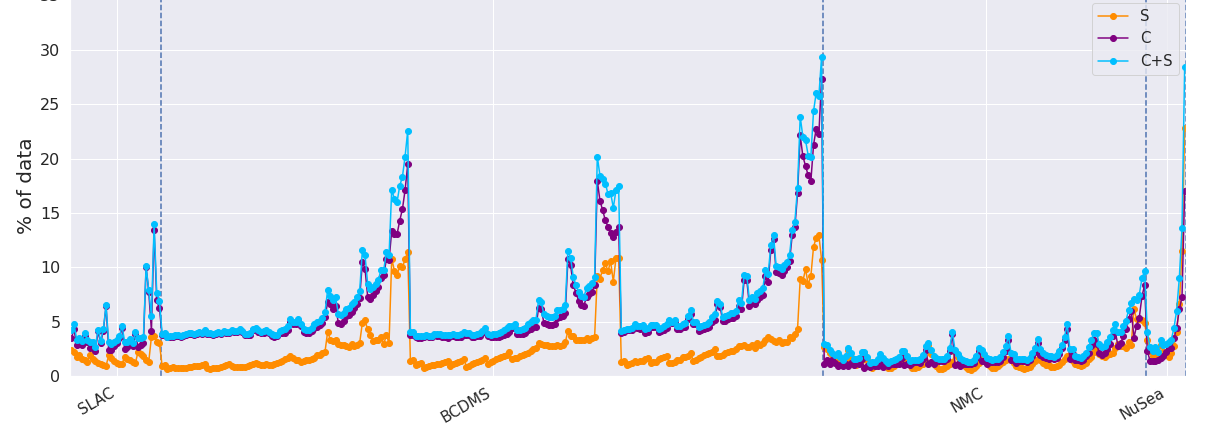
\includegraphics[width=85mm]{nuclear_uncs/diagdeut.png}
    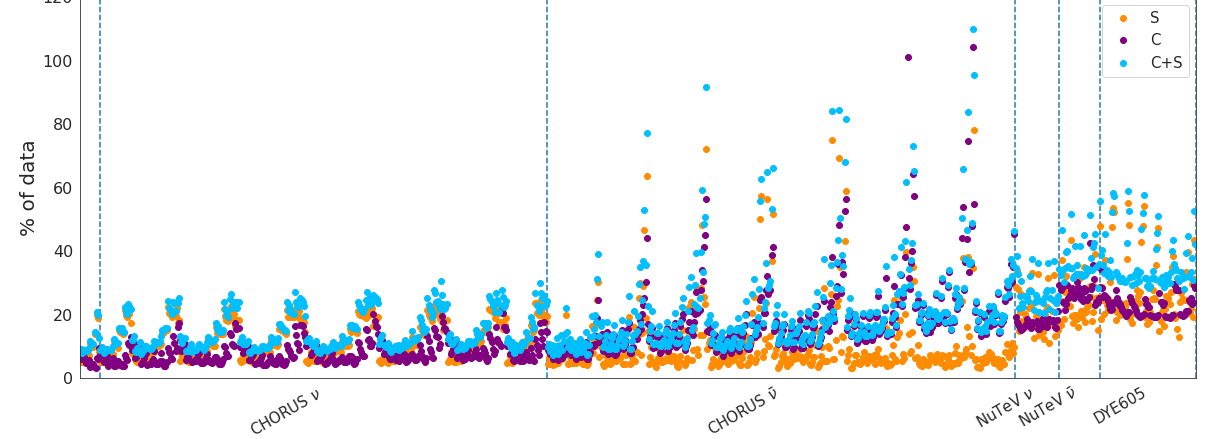
\includegraphics[width=85mm]{nuclear_uncs/diagnuc.png}
  \end{figure}
\end{frame}


%%%%%%%%%%%%%%%%%%%%%%%
\section{PDF properties and their implementation}
\author[Felix Hekhorn]{}
\institute{University of Milan}

\newcommand{\mmsbar}{{\overline{\rm {MS}}}}
\newcommand{\msbar}{$\mmsbar$}
\definecolor{UniSec6}{RGB}{50,110,30}
\providecommand{\iRef}[1]{{\tiny\color{UniSec6} $[$#1$]$}}

\subsection{PDF Positivity (TH)}

\begin{frame}{Positivity - Theory}
A. Candido, S. Forte, \underline{F. Hekhorn} \iRef{JHEP 11 (2020) 129}\\
{\bf Can \msbar{} parton distributions be negative?}\\
{\large \hfill \bf No!}

DIS: $F = \sum_j c_j \otimes f_j$

LO: Structure Function = PDF \checkmark

gluon@NLO:\\
\newcolumntype{e}{>{\centering\arraybackslash} m{.5\linewidth} }
\begin{tabular}{ee}
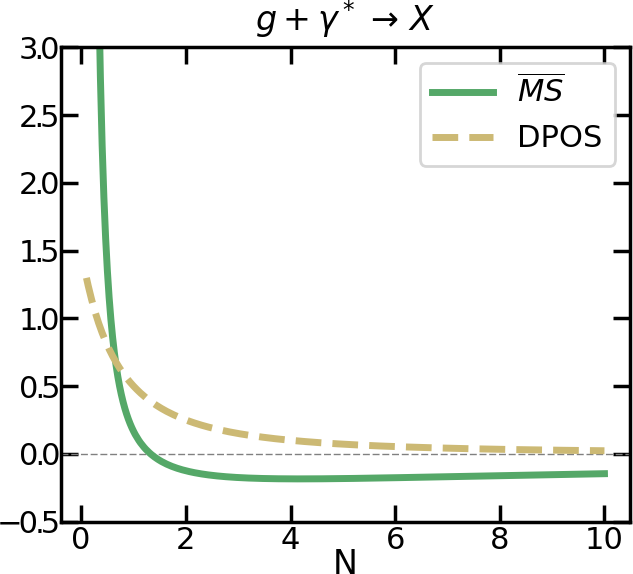
\includegraphics[height=4cm]{felix_positivity/disg.png}
&
\begin{itemize}
\item $c_g^{(1), bare}(z,Q^2,\epsilon) > 0$ \checkmark
\item $c_g^{(1), \mmsbar}(z) < 0$ for $z \to 1$
\item $c_g^{(1), \rm{DPOS}}(z) > 0$ \checkmark
\item $c_g^{(1), \rm{DIS}}(z) = 0$ \checkmark
\end{itemize}
\end{tabular}

\end{frame}

\begin{frame}{Positivity - Theory}
\begin{center}
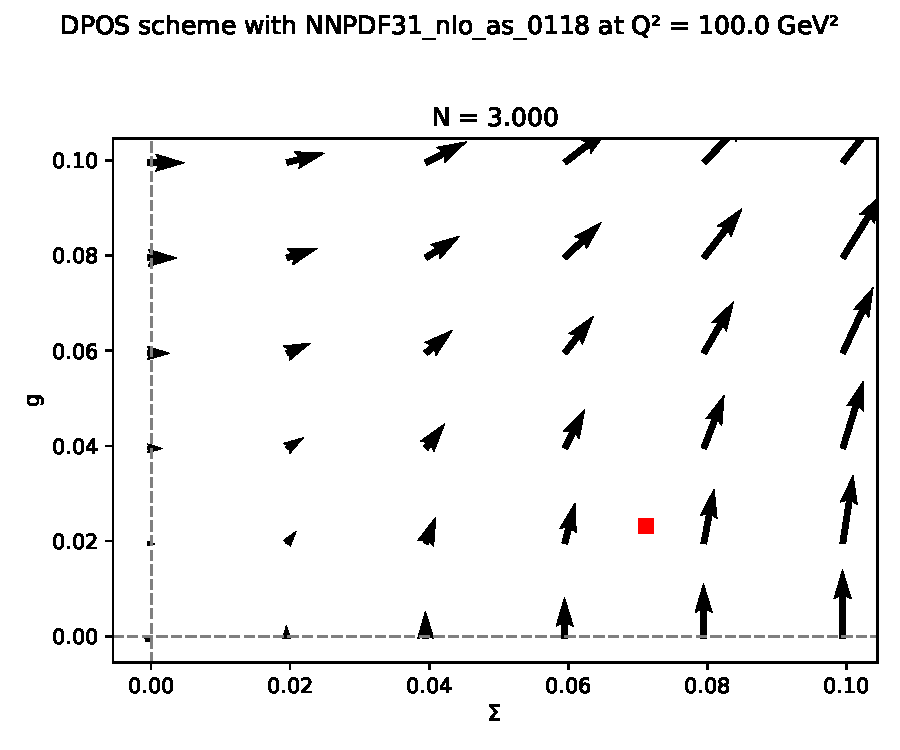
\includegraphics[height=5cm]{felix_positivity/quiver2-NNPDF31_nlo_as_0118-100_0-tiny-8.pdf}
\end{center}
\vspace{-2pt}
DPOS $\to$ \msbar: for $z < 1$ use perturbativity, for $z\to 1$ use \textit{exact} transformation $\Rightarrow \mmsbar > 0$\\
To obtain a physical xs/PDF is positivity {\bf sufficient?} no!\\
\hspace{149pt} or even {\bf necessary?} no!\\
$\Rightarrow$ but we can prove they \textit{are} positive and so it adds a cut in PDF space!
\end{frame}


\author[Tommaso Giani]{}
\institute{Nikhef}
\subsection{PDF Positivity (PH)}

\begin{frame}{Positivity - Implementation}
	Quarks, anti-quarks and gluon $\overline{MS}$ PDFs $q_k$ have to be positive: we add a term in the $\chi^2$ penalizing negative distributions
	\begin{align*}
		\label{eq:chi2pos_integ}
		\chi^2_{tot} = \chi^2_{exp} + \sum_k\, \chi^2_{k,\text{pos}}\,,
	\end{align*}

	\begin{align*}
		\chi^2_{k,pos} = \Lambda_k \,\sum_i \,\Theta\left(-q_k\left(x_i,Q^2\right)\right)\,,\,\,\,\,\,\,
		\text{with}\,\,\,\,\,\,\,
		\Theta\left(t\right) = 
		\begin{cases}
			t \,\,\,\,\,\,\text{if}\,\,\,\, t>0 \\
			0\,\,\,\,\,\,\,\text{if}\,\,\,\, t<0
		\end{cases}\,.
	\end{align*} 
	\begin{figure}[h!]
		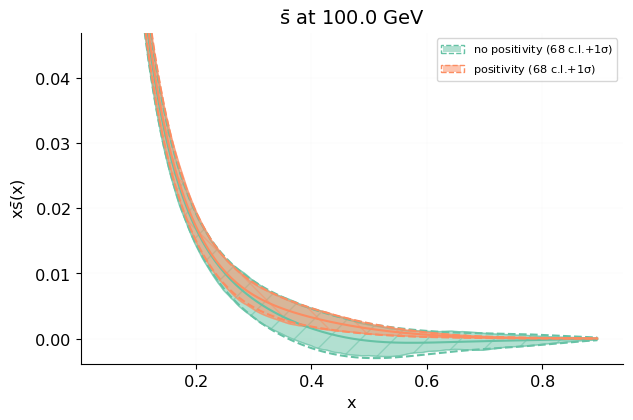
\includegraphics[scale=0.32]{pos_integ/plot_pdfs_bars_pos.png}
		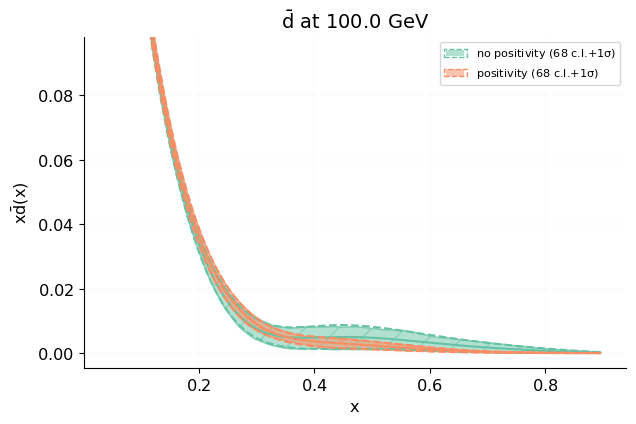
\includegraphics[scale=0.32]{pos_integ/plot_pdfs_bard_pos.png}
	\end{figure}
\end{frame}


\subsection{Integrability}
\begin{frame}{Integrability}
	In order to satisfy valence and Gottfried sum rules the distributions $ q_k =V, V_3, V_8, T_3, T_8$ have to be integrable at small-$x$
	\begin{align*}
		\lim_{x\rightarrow 0} xq_k\left(x,Q_0^2\right) = 0\,.%\,,\,\,\,\,\,\,\,\longrightarrow\,\,\,\,\,\,\, |xq_k|_{x\sim 0} \ll |xq_k|_{x=x_{\text{peak}}}
	\end{align*}
	Similarly to what done for positivity, we add to the total $\chi^2$ a penalty of the form
	\begin{align*}
		\chi^2_{k,integ} = \Lambda_k \,\sum_i \,\left[x_i\,q_k\left(x_i,Q^2\right)\right]^2\,.
	\end{align*}


	\begin{figure}[h!]
		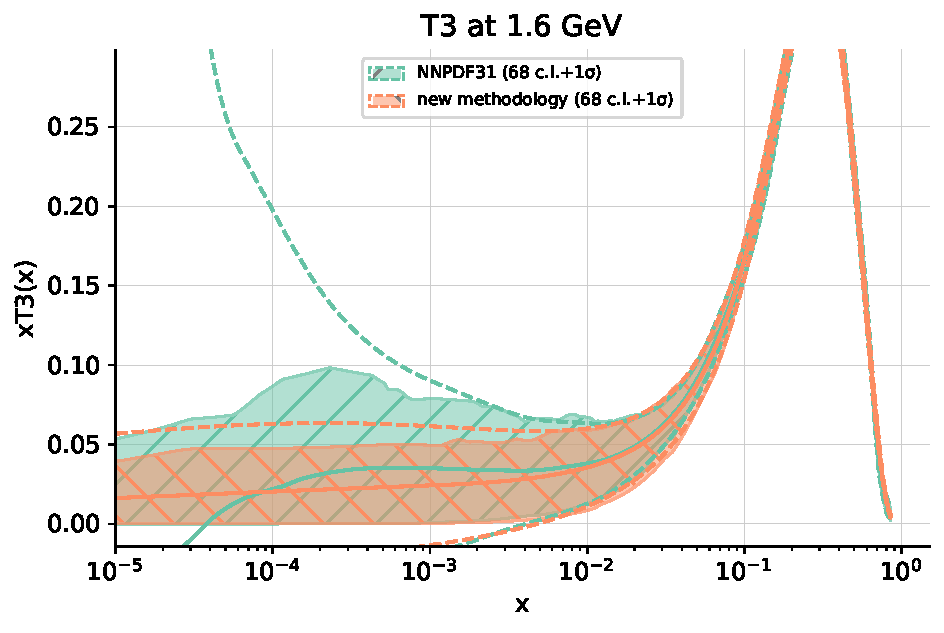
\includegraphics[scale=0.32]{pos_integ/plot_pdfs_T3_integ.pdf}
		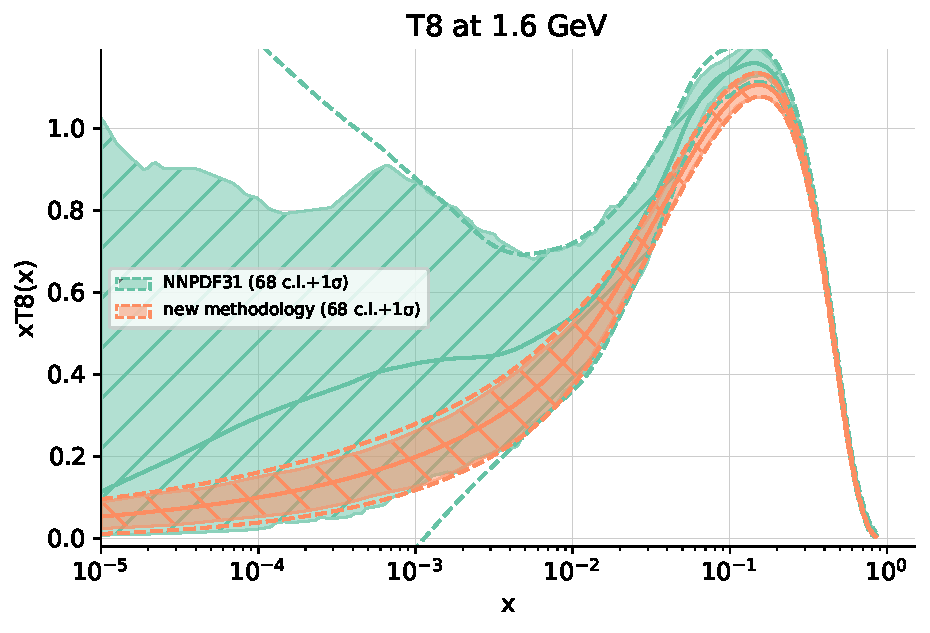
\includegraphics[scale=0.32]{pos_integ/plot_pdfs_T8_integ.pdf}
	\end{figure}

\end{frame}

\subsection{Architecture and fitbasis}
\begin{frame}{Fitbasis}
	\begin{columns}
		\begin{column}{0.55\textwidth}
			\begin{figure}[h!]
				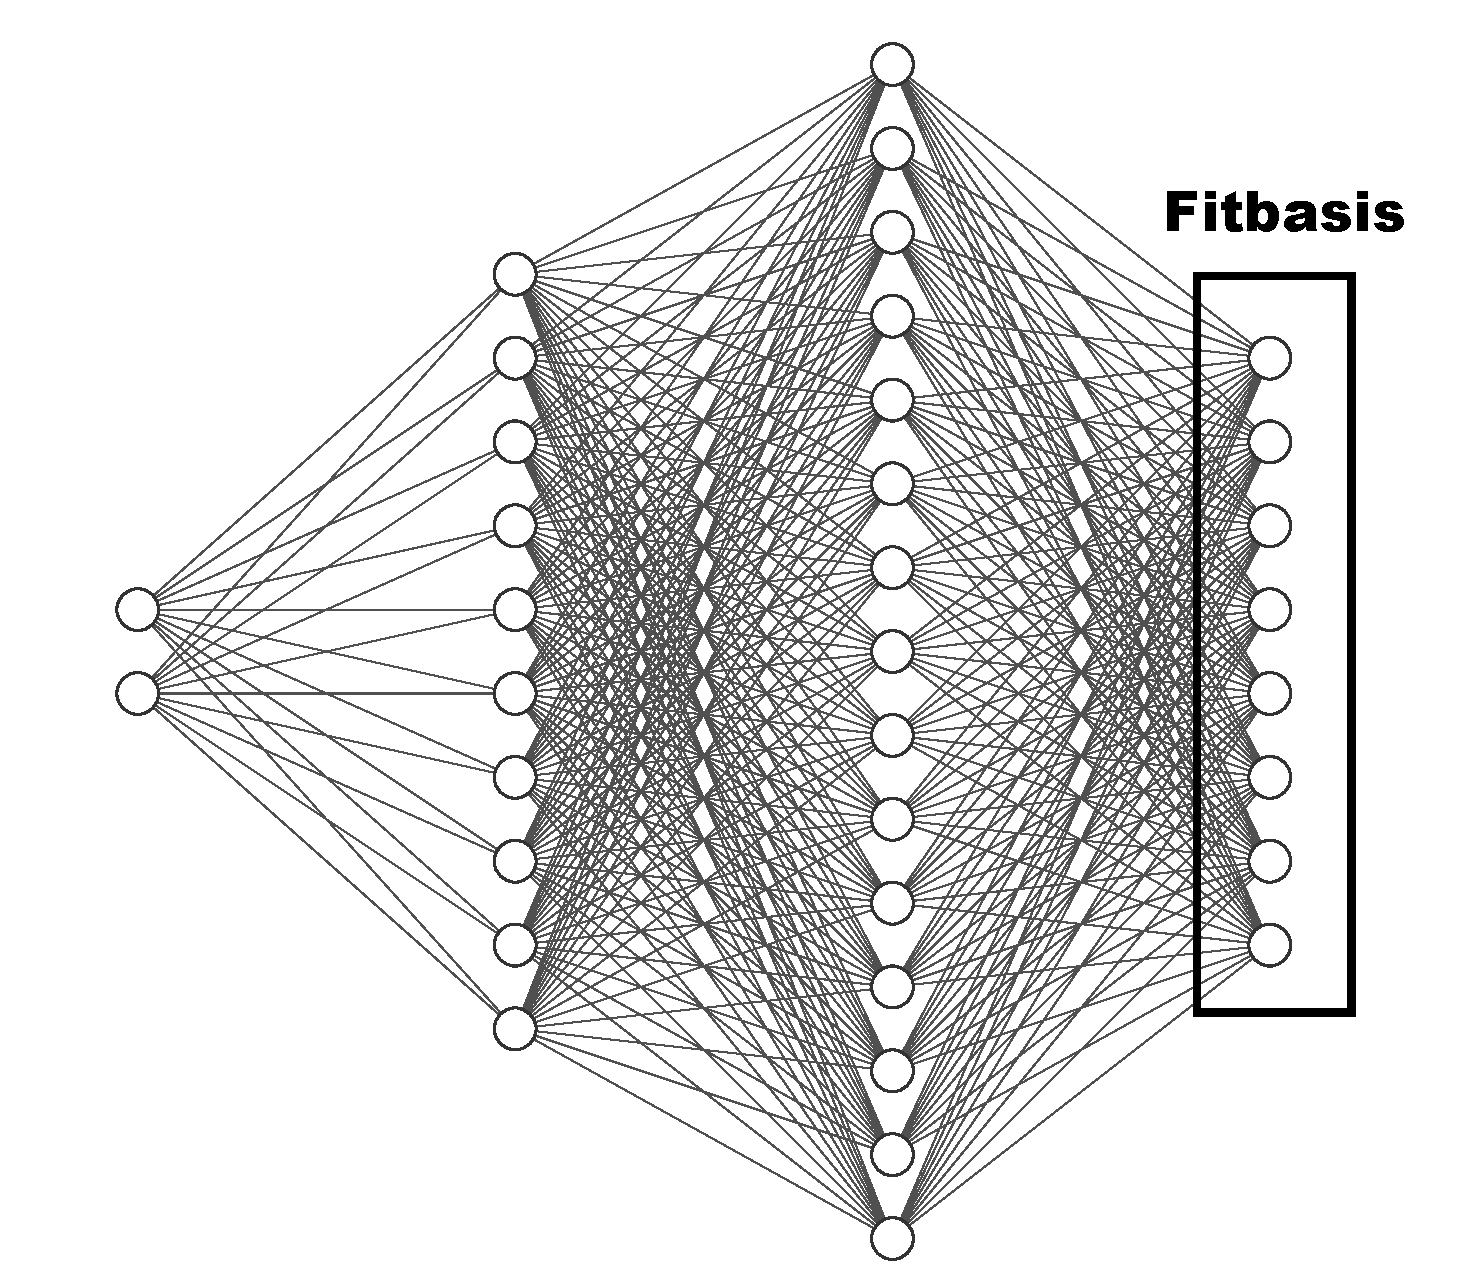
\includegraphics[scale=0.20]{pos_integ/output.pdf}
			\end{figure}
		\end{column}
		\begin{column}{0.45\textwidth}
			% Define block styles
		\tikzstyle{decision} = [diamond, draw, fill=blue!20, 
		text width=4.5em, text badly centered, node distance=3cm, inner sep=0pt]
	\tikzstyle{block} = [rectangle, draw,  
		text width=5em, text centered, rounded corners, minimum height=4em]
	\tikzstyle{line} = [draw, -latex']
	\tikzstyle{cloud} = [draw, ellipse,fill=red!20, node distance=3cm,
		minimum height=2em]
	\centering    
	\begin{tikzpicture}[node distance = 1.7cm]
		% Place nodes
		\node [block, text width=3.4cm] (FL) {\textbf{Flavour basis:} \\$g, u, \bar{u}, d, \bar{d}, s, \bar{s}, c$};
		\node [block, text width=5.0cm, below of=FL] (EV) {\textbf{Evolution basis:} \\$g, \Sigma, V, V_3, V_8, T_3, T_8, T_{15}$};
	\end{tikzpicture}
	\end{column}
\end{columns}
\begin{itemize}
	\item NNPDF4.0 will be hyper-optimized in the evolution basis \newline
	\item the final results should not depend on the details of the methodology \\
	$\rightarrow$ fitbasis independence studies \newline
	\item independently on the basis choice the same physical constraints have to be satisfied: positivity and integrability
\end{itemize}
\end{frame}





%%%%%%%%%%%%%%%%%%%%%%%
\section{PDF determination methodology}
\definecolor{darkgreen}{rgb}{0.0, 0.5, 0.13}
\newcommand{\gct}{\color{darkgreen}\checkmark}
\newcommand{\rma}{\color{red}\ding{55}}
\newcommand{\bct}{\color{blue}\checkmark}

\author[Juan Cruz-Martinez]{}
\institute{University of Milan}

\subsection{Hyperoptimization and K-folding}

\begin{frame}{Beyond the PDF fit: fitting the methodology}

    The main objective of NNPDF is to minimize choices that can bias the PDF:

    \begin{columns}
        \column{0.7\linewidth}
        \begin{itemize}
            \item[\rma] Functional form $\longrightarrow$ Neural Networks
            \item[\rma] However: NN are defined by set of parameters!
        \end{itemize}

        \vspace{0.2cm}

        Humans are good at recognising patterns but selecting the best
        set of parameters is a slow process and systematic success is not guaranteed
        \column{0.2\linewidth}
        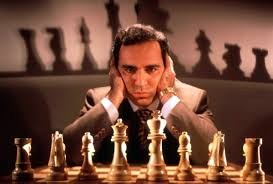
\includegraphics[width=\textwidth]{juan_future_hyperopt/kasparov.jpg}

        
\includegraphics[width=\textwidth]{juan_future_hyperopt/alphazero.jpg}
        \column{0.1\linewidth}
    \end{columns}

    \vspace{0.2cm}

    To overcome this selection problem we implement a {\color{blue}  hyperparameter scan}: let the computer decide automatically

    \begin{itemize}
        \item[\gct] Scan over thousands of hyperparameter combinations
        \item[\gct] Define a reward function to grade the model
        \item[\gct] Check the generalization power of the model
    \end{itemize}

\end{frame}

\begin{frame}
    \frametitle{Hyperparameter scan} 
    Each blue dot corresponds to a fit of a different set of hyperparameters:
    { 
        \centering 

        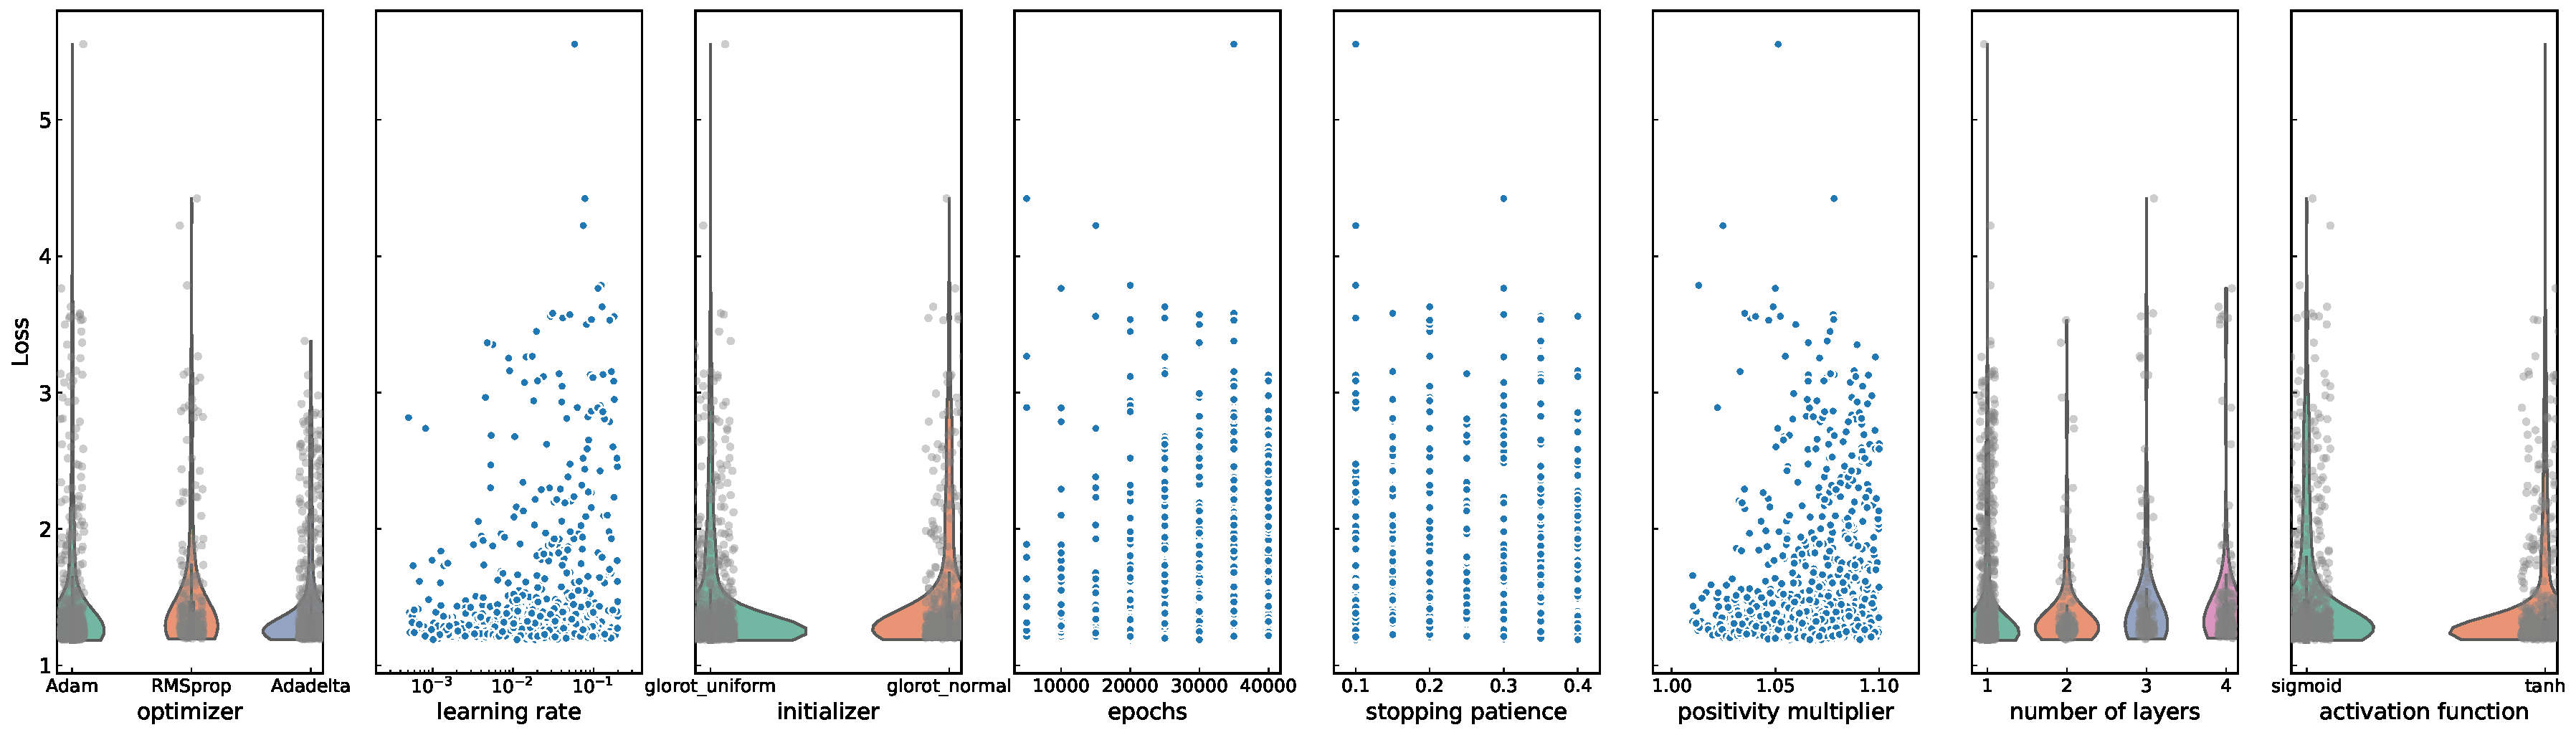
\includegraphics[width=\textwidth]{juan_future_hyperopt/dis-fullpage.pdf}
        Thousands of fits for the hyperoptimization algorithm to choose:

        \begin{columns} \small
            \column{0.35\paperwidth}
            \begin{itemize}
                \item[\bct] Optimizer
                \item[\bct] Initializer
                \item[\bct] Stopping Patience
                \item[\bct] Number of Layers
            \end{itemize}
            \column{0.35\paperwidth}
            \begin{itemize}
                \item[\bct] Learning Rate
                \item[\bct] Epochs
                \item[\bct] Positivity Multiplier
                \item[\bct] Activation Function
            \end{itemize}
        \end{columns}
    } \vfill
\end{frame}

\begin{frame}
    \frametitle{Hyperoptimization: reward and generalization}
    If we use as hyperoptimization target the $\chi^{2}$ of the fitted data, we risk finding the hyperparameter set that
    better overfits.


    \vfill

    \begin{columns}
        \column{0.75\linewidth}
        We avoid this problem by adopting \textbf{$\boldsymbol{k}$-folding}:

        \begin{itemize}
            \item Divide the data into $k$ sets.
            \item Leave one set out and fit the $k-1$ sets left.
            \item Optimize the average $\chi^{2}$ of the $k$ non-fitted sets.
        \end{itemize}
        \column{0.25\linewidth}
        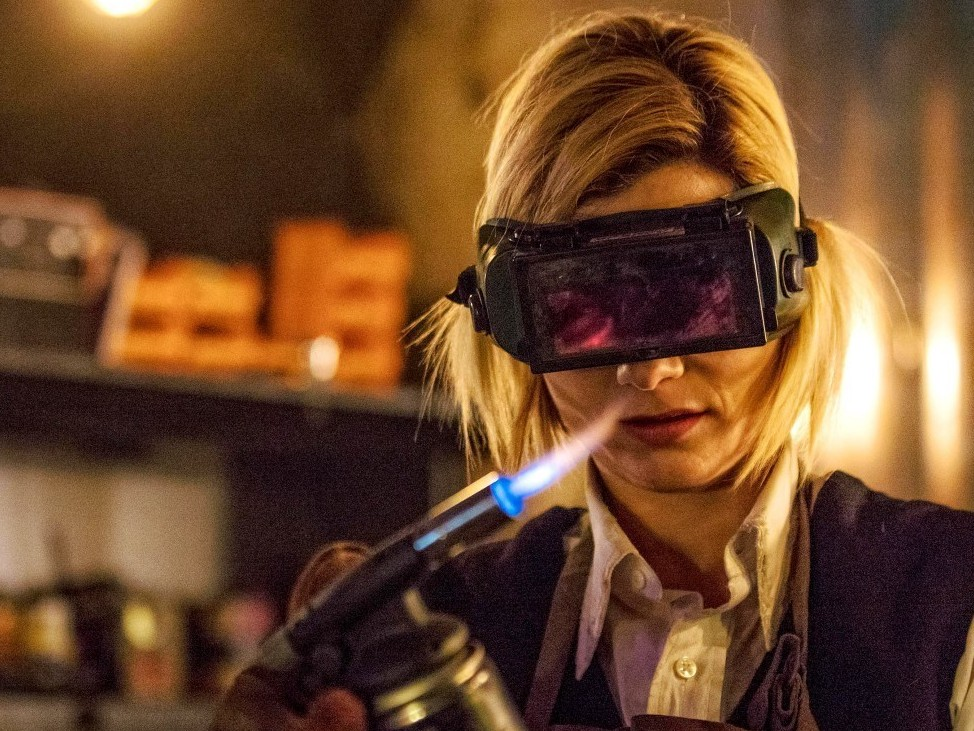
\includegraphics[width=\textwidth]{juan_future_hyperopt/doctor.jpg}
    \end{columns}

    \vspace{0.4cm}

    Example of function to hyperoptimize:

    \begin{equation*}
        \text{Loss}(optimizer\_name,\ depth\_of\_network) = \frac{1}{k}\displaystyle\sum^{i}_{k} \frac{\chi^{2}_{i}}{N_{i}}
    \end{equation*}

    Where we are computing the $\chi^{2}$ for the data that did not enter the fit. This ensures that the methodology
    can accommodate well even data that has never been seen by the fit.

\end{frame}

\definecolor{darkgreen}{rgb}{0.0, 0.5, 0.13}
\newcommand{\gct}{\color{darkgreen}\checkmark}
\newcommand{\rma}{\color{red}\ding{55}}
\newcommand{\bct}{\color{blue}\checkmark}
\title{NNPDF}
\author[Roy Stegeman]{}
\institute{University of Milan}
\date{PDF4LHC}

\subsection{Correlation and combination of PDF sets}

\begin{frame}{Self-correlation of PDF sets}
    	\begin{columns}[t]
        	\column{0.5\linewidth}
        	
		 Are PDF sets based on the same NNPDF methodology and underlying data fully correlated with respect to the data replicas?

        	\vspace{0.2cm}
			No, they are not fully correlated as a result of uncorrelated functional uncertainties.

		\vspace{0.2cm}
			\only<2>{If the correlation is higher, this means the functional uncertainty is smaller if compared to the data uncertainty.}

        	\column{0.5\linewidth}
        		\begin{center}
        		\begin{figure}
            		\captionsetup{format=smol}
            		\includegraphics<1>[width=\textwidth]{roy_pdf_correlations/nnpdf31_corr.pdf}
            		\includegraphics<2>[width=\textwidth]{roy_pdf_correlations/nnpdf31&40_corr.pdf}
            		\vspace{-0.9cm}
            		\caption{\tiny PDF-PDF self-correlation calculated with respect to data replicas, for sets based on the same NNPDF methodology and data, but different (random) initialization}        		
			\end{figure}
			\end{center}

    	\end{columns}
\end{frame}


\begin{frame}{Combination of PDF sets}
    	\begin{columns}[t]
        	\column{0.6\linewidth}

			At present PDF sets are combined under the assumption that they are fully correlated, can we instead combine the PDF sets in a correlated way?

        	\vspace{0.2cm}
			No, this can lead to arbitrarily small uncertainties if we combine repeated PDF determinations.

       	\column{0.4\linewidth}
       	\vspace{-2.7cm}
       	\begin{center}
       		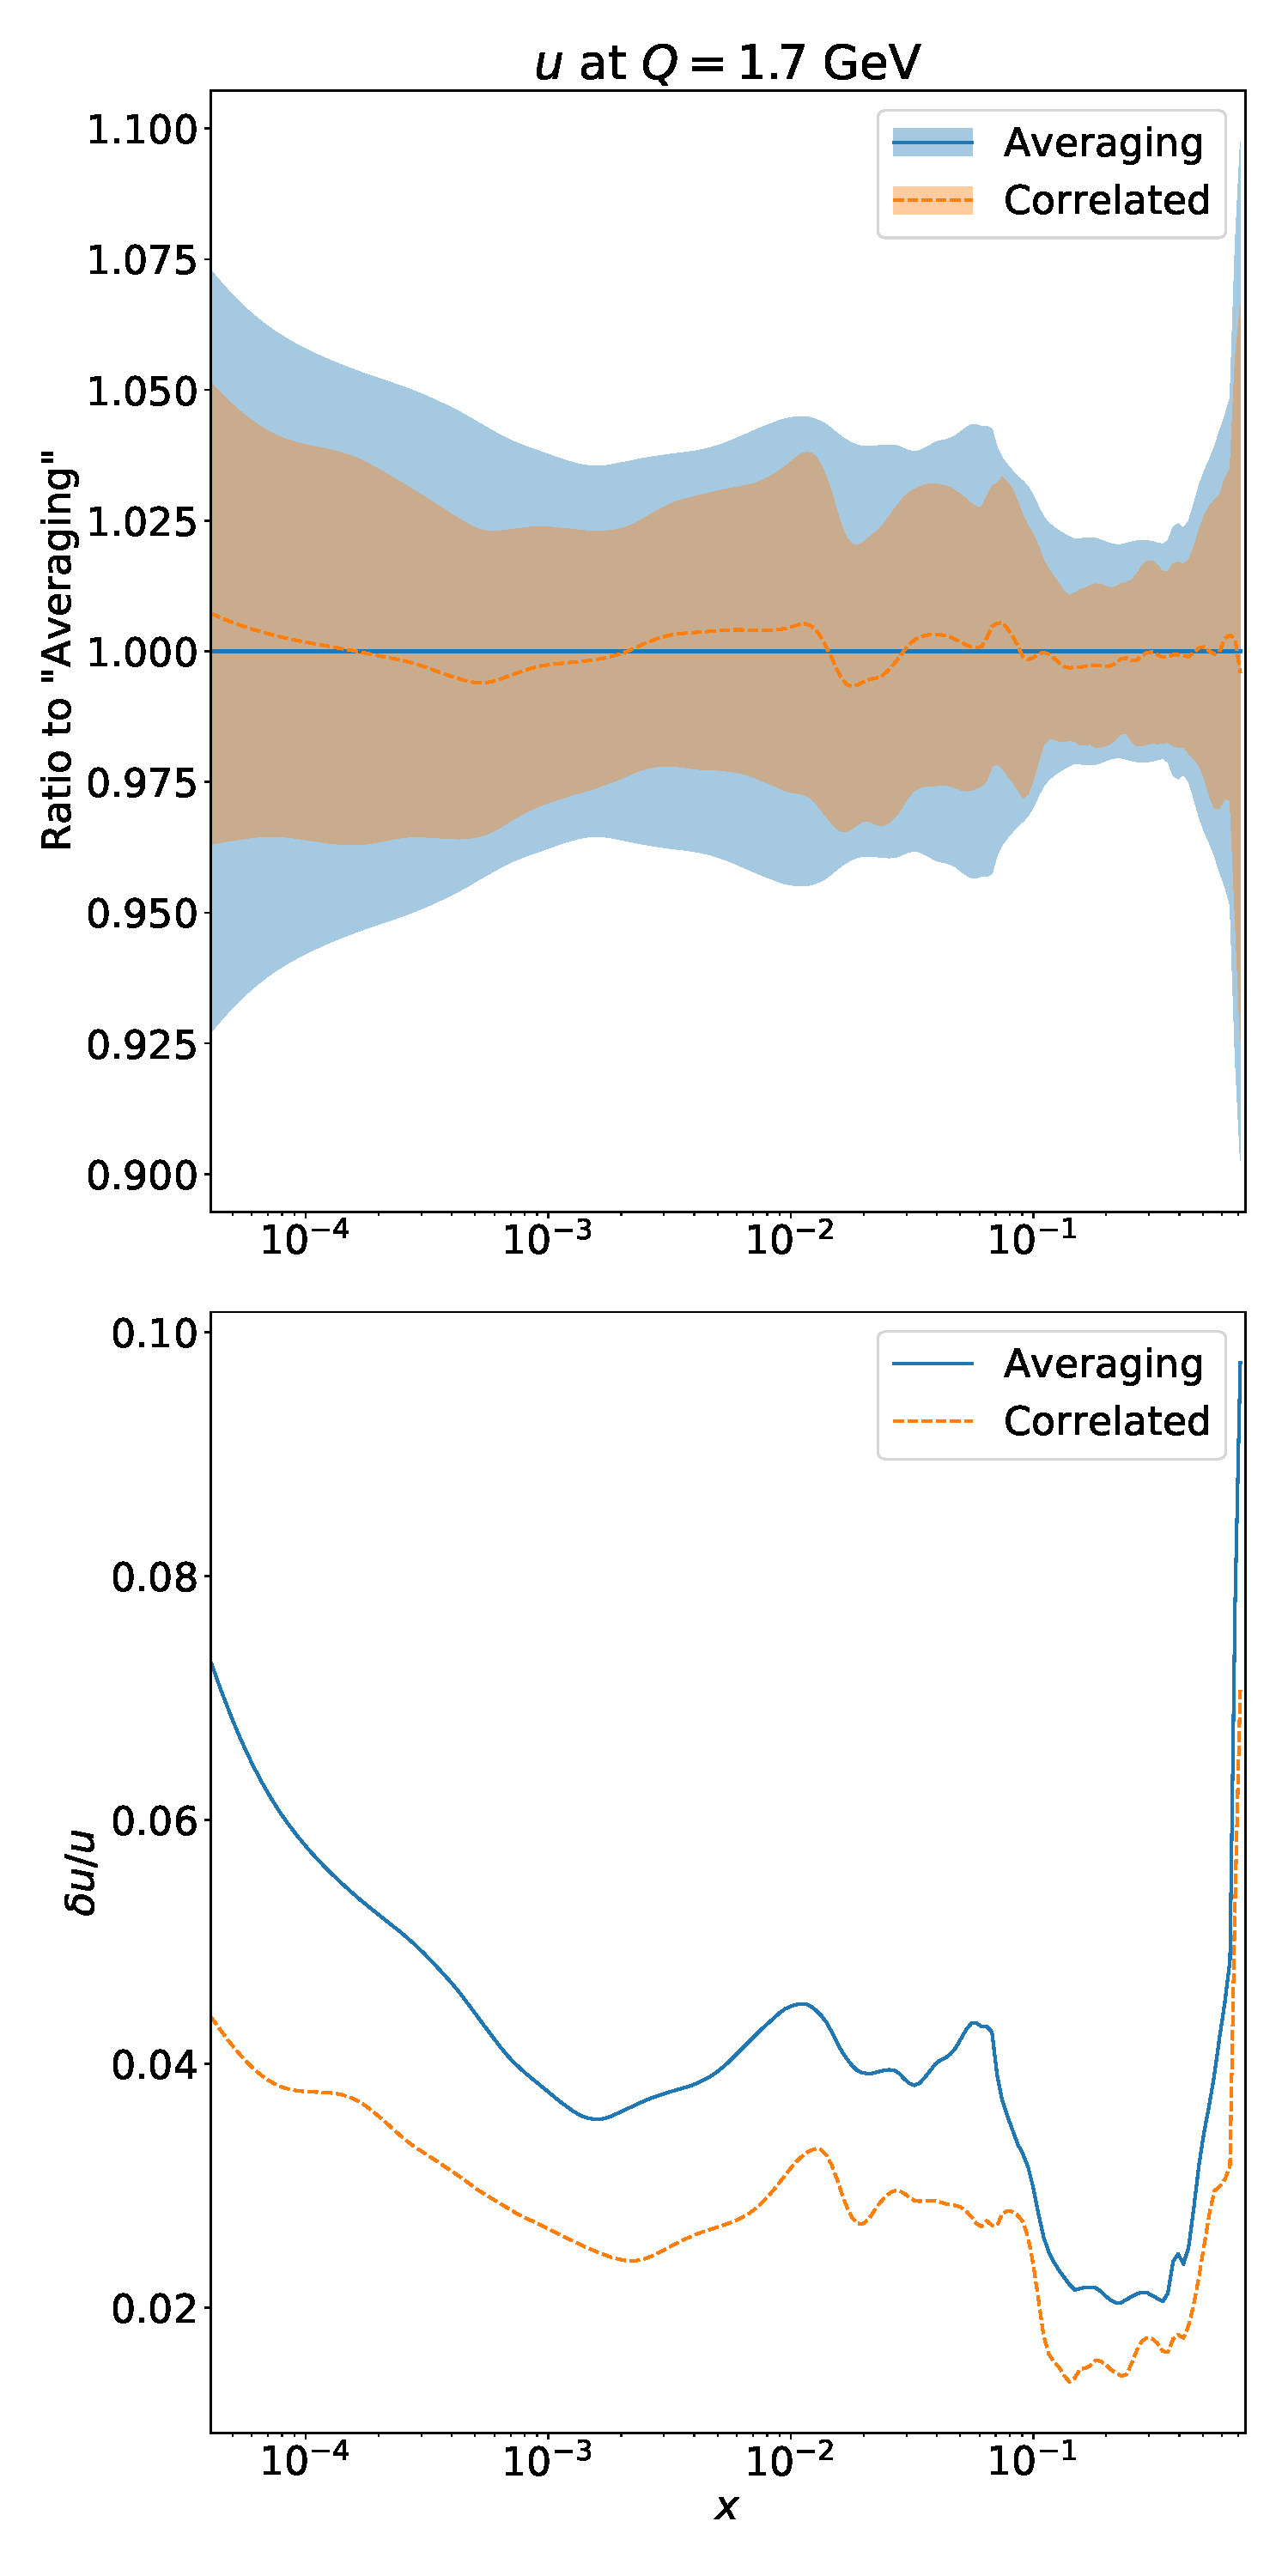
\includegraphics[height=1.15\textheight]{roy_pdf_correlations/ratio_2.pdf}
       	\end{center}
			
    	\end{columns}
\end{frame}



%%%%%%%%%%%%%%%%%%%%%%%
\section{PDF validation}
\newcommand{\shift}{\eta}
\newcommand{\vv}[1]{\boldsymbol{#1}}
\newcommand{\erep}{\mathbf{E}_{\epsilon}}
\newcommand{\eshift}{\mathbf{E}_{\shift}}
\newcommand{\ndata}{N_{\rm data}}
\newcommand\Fontvi{\fontsize{8}{7.2}\selectfont}

\makeatletter
\newcommand{\leqnomode}{\tagsleft@true\let\veqno\@@leqno}
\newcommand{\reqnomode}{\tagsleft@false\let\veqno\@@eqno}
\makeatother

\title{NNPDF}
\author[Michael Wilson]{Christopher Schwann and Rosalyn Pearson and Michael Wilson}
\institute{University of Edinburgh}
\date{PDF4LHC}

\subsection{Closure testing NNPDF4.0}
\begin{frame}
    \frametitle{Closure Test}
    \Fontvi
    \begin{columns}[t]
    \column{0.5\textwidth}
    Fit replicas to pseudodata in usual way
    \leqnomode
    \begin{equation}\label{eq:dataassum}
    \begin{split}
        \vv{y} &= \vv{f} + \vv{\shift} + \vv{\epsilon} \\
        &= \vv{z} + \vv{\epsilon},
    \end{split}
    \end{equation}
    where $\vv{\shift} \sim \mathcal{N}(0, C)$ and $\vv{\epsilon} \sim \mathcal{N}(0, C)$ are sampled independently.
    
    Use predictions from an input PDF as proxy for $\vv{f}$.

    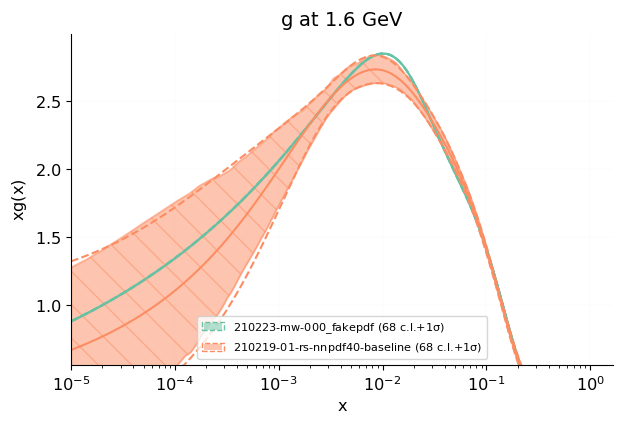
\includegraphics[scale=0.3]{closure_test/plot_pdfs_g.png}
    
    Sampling a random NNPDF replica as the input PDF for a closure test.
    \column{0.5\textwidth}
    \reqnomode
    Allows testing of methodology, if the input assumptions hold.

    \vspace{8pt}
    For example:
    \vspace{8pt}
    
    \textbf{Bias}: difference between central prediction and true observable

    \vspace{8pt}
    \textbf{Variance}: uncertainty of replica predictions

    \vspace{8pt}
    
    Bias is a stochastic variable. If PDF uncertainty is faithful then
    \begin{equation}
        \eshift[{\rm bias}] = {\rm variance}
    \end{equation}

    \vspace{8pt}
    
    High demand on resources - made feasible with \texttt{n3fit}
    \end{columns}
\end{frame}
%
\begin{frame}\frametitle{Preliminary results}
    \Fontvi
    Compare first moments:

    \begin{center}
    \begin{tabular}{lr}
        \toprule
        {} &  $\sqrt{\eshift[{\rm bias}] / \eshift[{\rm variance}]}$\\
        \midrule
        Total      & 1.11 $\pm$ 0.5 \\
        \bottomrule
        \end{tabular}
    \end{center}

    \vspace{8pt}
    Alternatively look at the respective distributions

    \vspace{8pt}
    \begin{center}
        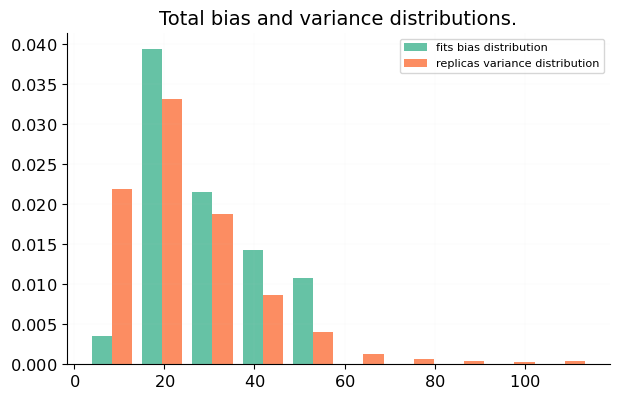
\includegraphics[scale=0.3]{closure_test/plot_bias_variance_distributions_3.png}
    \end{center}

    \vspace{8pt}
    Bias distribution sampled with 25 fits, 40 replicas each.

\end{frame}
\newcommand{\hlme}[1]{{\color{red}\bf #1}}

\author[Juan Cruz-Martinez]{}
\institute{University of Milan}

\subsection{Back to the future}

\begin{frame}{How can we future-proof the methodology?}{Do we trust our errorbands?}

    \small
    The smaller error bands in the NNPDF4.0 fits are driven both by the increased amount of data and the
    improved methodology.
    But there are still kin. regions not covered by data!

    \begin{columns}
        \column{0.6\linewidth}
        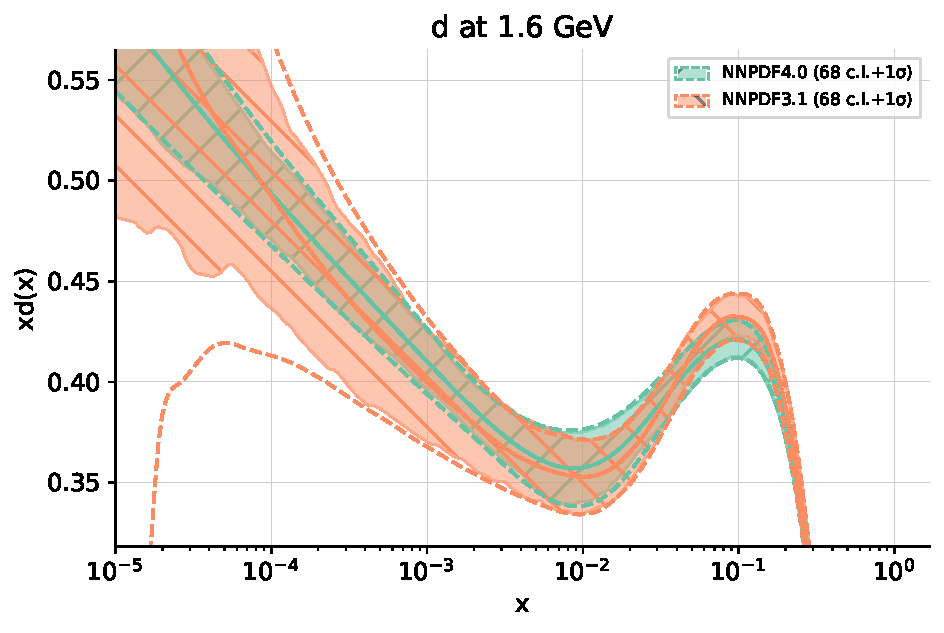
\includegraphics[width=1.0\textwidth]{juan_future_hyperopt/dquark.pdf}

        \column{0.4\linewidth} \vspace{-2.3cm} {

            Ideally: design an experiment for the regions not covered by fitted-data!

            \vspace{0.3cm}

            Problem: we want the results before 2050...

        }
    \end{columns}

    \vspace{-0.3cm}

    \begin{columns}
        \column{0.7\linewidth}
        Solution: chronologically ordered subsets of data to test unseen regions, we named this ``future tests``.

        \column{0.3\linewidth}
        \vspace{-1.9cm}
        \begin{figure}
            \captionsetup{format=smol}
            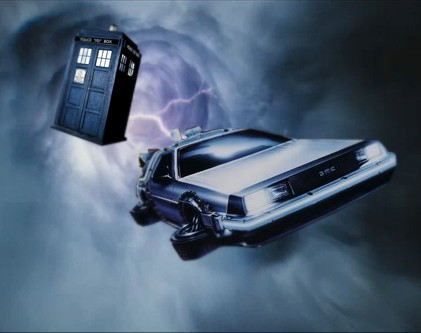
\includegraphics[width=0.7\textwidth]{juan_future_hyperopt/tardisdelorean.jpg}
            \caption{\tiny Other valid and certified future-testing methods}
        \end{figure}
    \end{columns}



\end{frame}


\begin{frame}{Future tests}{for more information see \href{https://arxiv.org/pdf/2103.08606.pdf}{\color{blue} arxiv:2103.08606}}

    \begin{columns}
        \column{0.60\linewidth}
        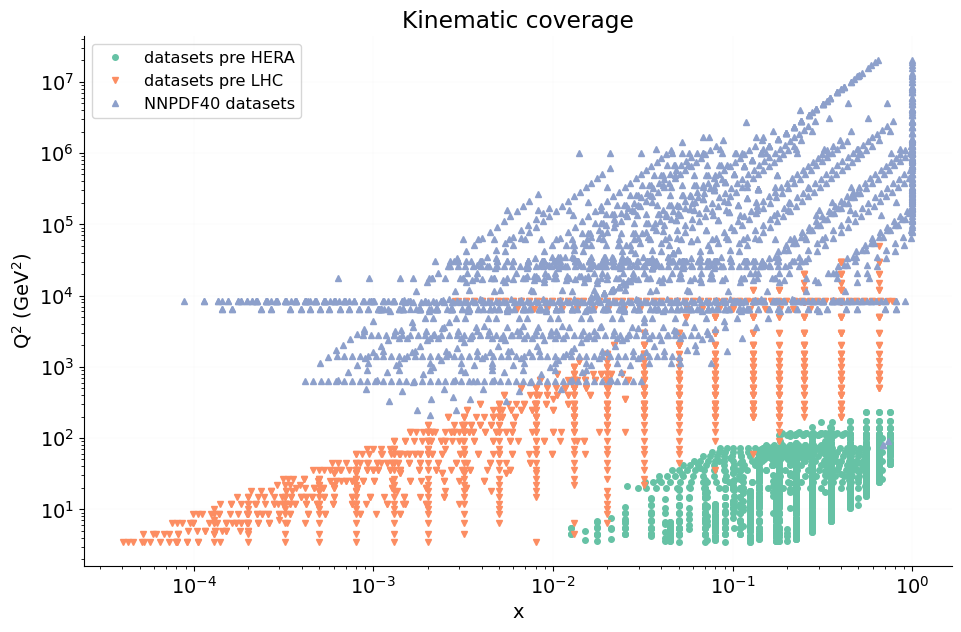
\includegraphics[width=\textwidth, height=0.8\textheight]{juan_future_hyperopt/kincov.png}
        \column{0.46\linewidth}
        \vspace{-0.9cm}
        \only<1>{
            \begin{table}
                \tiny
                \centering
                \caption*{\scriptsize $\chi^{2}/N$ (only exp. covmat)}
                \begin{tabular}{c | c c c} \toprule
                    (dataset) & NNPDF4.0 & pre-LHC & pre-Hera  \\ \midrule
                    pre-HERA  & 1.09 & 1.01 & 0.90 \\
                    pre-LHC   & 1.21 & 1.20 & \hlme{23.1} \\
                    NNPDF4.0  & 1.29 & \hlme{3.30} & \hlme{23.1} \\
                    \bottomrule
                \end{tabular}
            \end{table}
        }
        \only<2>{
            \begin{table}
                \tiny
                \centering
                \caption*{\scriptsize $\chi^{2}/N$ (exp. and PDF covmat)}
                \begin{tabular}{c | c c c} \toprule
                    (dataset) & NNPDF4.0 & pre-LHC & pre-Hera  \\ \midrule
                    pre-HERA  &  & & 0.86 \\
                    pre-LHC   &  & 1.17 & \hlme{1.22} \\
                    NNPDF4.0  & 1.12 & \hlme{1.30} & \hlme{1.38} \\
                    \bottomrule
                \end{tabular}
            \end{table}
        }


        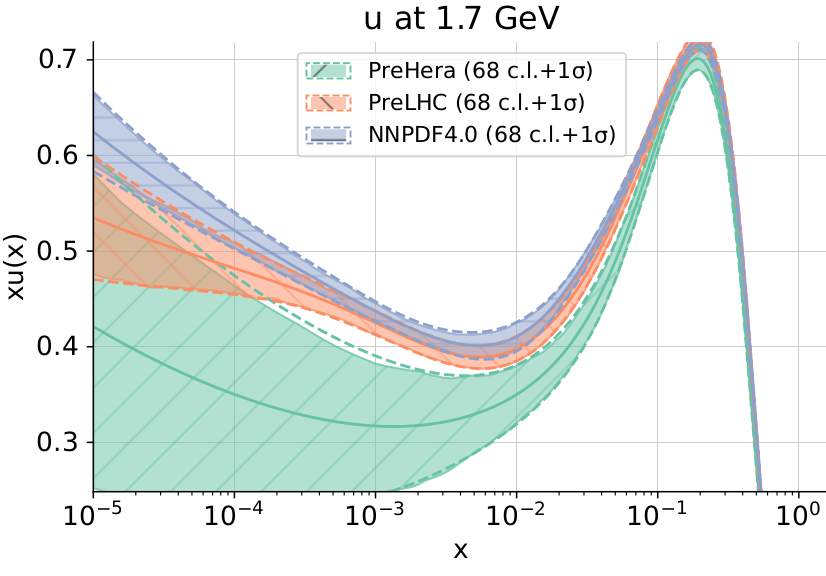
\includegraphics[width=1.0\textwidth]{juan_future_hyperopt/diffu}

    \end{columns}
\end{frame}


%%%%%%%%%%%%%%%%%%%%%%%
\section{Dataset selection}
\author[Zahari Kassabov]{}
\institute{University of Cambridge}
\subsection{Weighted PDFs}
\begin{frame}{Why can't we fit a dataset?}
\protect\hypertarget{why-cant-we-fit-a-dataset}{}
Three possibilities:

\begin{enumerate}
\tightlist
\item
  Problems with the experiment
\item
  Problems with the theory (including methodology)
\item
  Tension with other dataset (i.e.~1. or 2. but for other data)
\end{enumerate}

\textbf{Objective}: Investigate the origin of issue

\textbf{Tool: Constrained fits}; Try to constrain the fit to agree with
the dataset under investigation and see what breaks in the process.
\end{frame}

\begin{frame}{Implementation}
\protect\hypertarget{implementation}{}
Idea from \emph{Why \(\alpha_s\) Cannot be Determined from Hadronic
Processes without Simultaneously Determining the Parton Distributions}
{[}Forte, Z.K.,
\href{https://arxiv.org/abs/2001.04986}{\textbf{arxiv:2001.04986}}{]}

Instead of optimizing for the total \(\chi^2\), give special attention
to the agreement of the dataset under investigation by giving more
weight to its error \(\chi^2_p\).

\[
\chi^2 + w \chi^2_p
\] where \(w\) is \emph{big}.

Consequences, compared to optimizing for \(\chi^2\):

\begin{itemize}
\tightlist
\item
  Total \(\chi^2\) will go up, because we are not optimizing for it any
  longer.

  \begin{itemize}
  \tightlist
  \item
    Observe which datasets get worse and how much: Assess \textbf{3}.
  \end{itemize}
\item
  Dataset error, \(\chi^2_p\) will go down.

  \begin{itemize}
  \tightlist
  \item
    Observe if we can reasonably get a good agreement or the dataset is
    not self consistent. Conclude \textbf{1} or \textbf{2}, but likely
    \textbf{1} as our methodology is \emph{very} flexible
  \end{itemize}
\end{itemize}
\end{frame}

\begin{frame}{Example: DO electron Asymmetry}
\protect\hypertarget{example-do-electron-asymmetry}{}
We cannot fit the D0 electron assymetry dataset. Set $w=411$.

\tiny
\begin{longtable}[]{@{}lll@{}}
\toprule
\begin{minipage}[b]{0.19\columnwidth}\raggedright
\(\chi^2\)/ndat\strut
\end{minipage} & \begin{minipage}[b]{0.14\columnwidth}\raggedright
Baseline\strut
\end{minipage} & \begin{minipage}[b]{0.28\columnwidth}\raggedright
Reweighted D0EASY\strut
\end{minipage}\tabularnewline
\midrule
\endhead
\begin{minipage}[t]{0.19\columnwidth}\raggedright
D0 e ASY\strut
\end{minipage} & \begin{minipage}[t]{0.14\columnwidth}\raggedright
5.3\strut
\end{minipage} & \begin{minipage}[t]{0.28\columnwidth}\raggedright
1.7\strut
\end{minipage}\tabularnewline
\begin{minipage}[t]{0.19\columnwidth}\raggedright
D0 \(\mu\) ASY\strut
\end{minipage} & \begin{minipage}[t]{0.14\columnwidth}\raggedright
2.0\strut
\end{minipage} & \begin{minipage}[t]{0.28\columnwidth}\raggedright
5.4\strut
\end{minipage}\tabularnewline
\begin{minipage}[t]{0.19\columnwidth}\raggedright
Total\strut
\end{minipage} & \begin{minipage}[t]{0.14\columnwidth}\raggedright
1.17\strut
\end{minipage} & \begin{minipage}[t]{0.28\columnwidth}\raggedright
1.29\strut
\end{minipage}\tabularnewline
\bottomrule
\end{longtable}
\vspace{-1.5em}

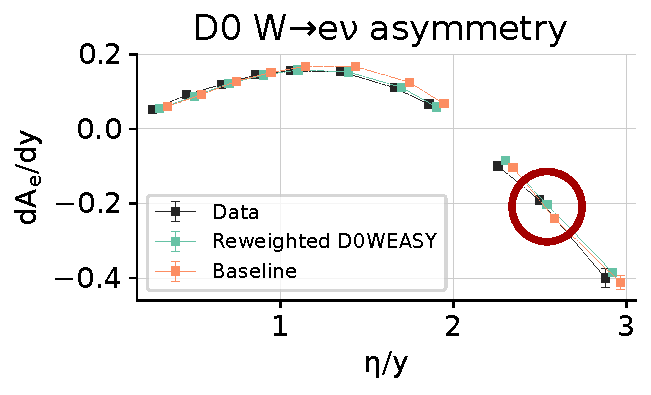
\includegraphics[width=0.45\textwidth,height=0.26\textwidth]{weight_fits/plots/D0WEASY_Norm1_plot_fancy_0.pdf}
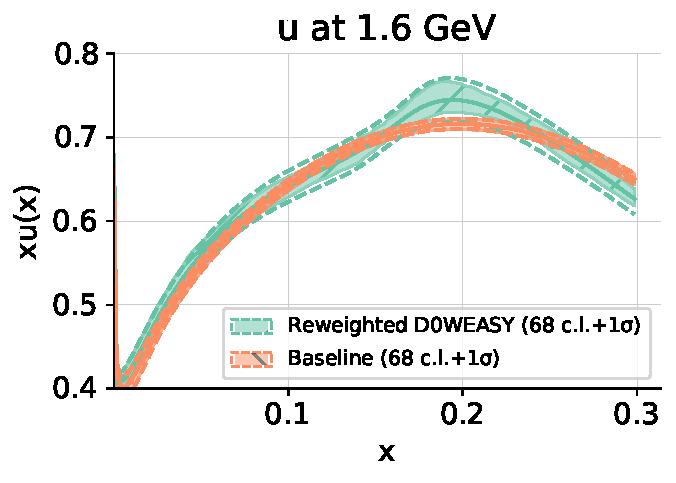
\includegraphics[width=0.45\textwidth,height=0.26\textwidth]{weight_fits/plots/plot_pdfs_u.pdf}
\normalsize


\vspace{-1em}

\begin{itemize}
\tightlist
\item
  Can lift the downward prediction but only at the cost of:

  \begin{itemize}
  \tightlist
  \item
    Introducing unnatural shapes
  \item
    Increasing error in other datasets particularly D0 \(\mu\)
    asymmetry.
  \end{itemize}
\item
  The large weight fit still obtains poor fit quality for D0EASY:

  \begin{itemize}
  \tightlist
  \item
    \textbf{Dataset not self consistent}.
  \end{itemize}
\end{itemize}
\end{frame}


%%%%%%%%%%%%%%%%%%%%%%%
\section{PDF delivery}
\definecolor{HallowGreen}{RGB}{50,110,30}
\providecommand{\iRef}[1]{{\tiny\color{HallowGreen} $[$#1$]$}}

\author[Tanjona Rabemananjara]{}
\institute{University of Milan}

\subsection{PDF replica compression}

\begin{frame}{Efficient PDF Compression with GANs}
	S. Carrazza, J. Cruz-Martinez, \underline{T. Rabemananjara} \iRef{arXiv (2021)} \\
	\textbf{\textcolor{HallowGreen}{\underline{Goal}:}} Provide a smaller set of MC 
	replicas that best represents the Probability Distribution of a given PDF set 
	with large samples.
	\vspace*{-0.1cm}	
	\begin{center}
	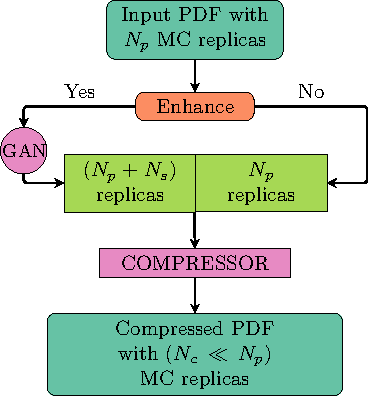
\includegraphics[height=.7\textheight]{./gan_compressor/imgs/pygans.pdf}
	\end{center}
\end{frame}

\begin{frame}{Efficient PDF Compression with GANs}
	\underline{Standard vs. GAN-Enhanced Compressor}:
	\begin{center}
		\textcolor{red}{\textbf{\underline{SETUP}:}} ($N_p=1000 + N_s=2000$) 
		$\longrightarrow$ $N_c$
	\end{center}
	\begin{columns}[T] 
	\begin{column}{.5\textwidth}
	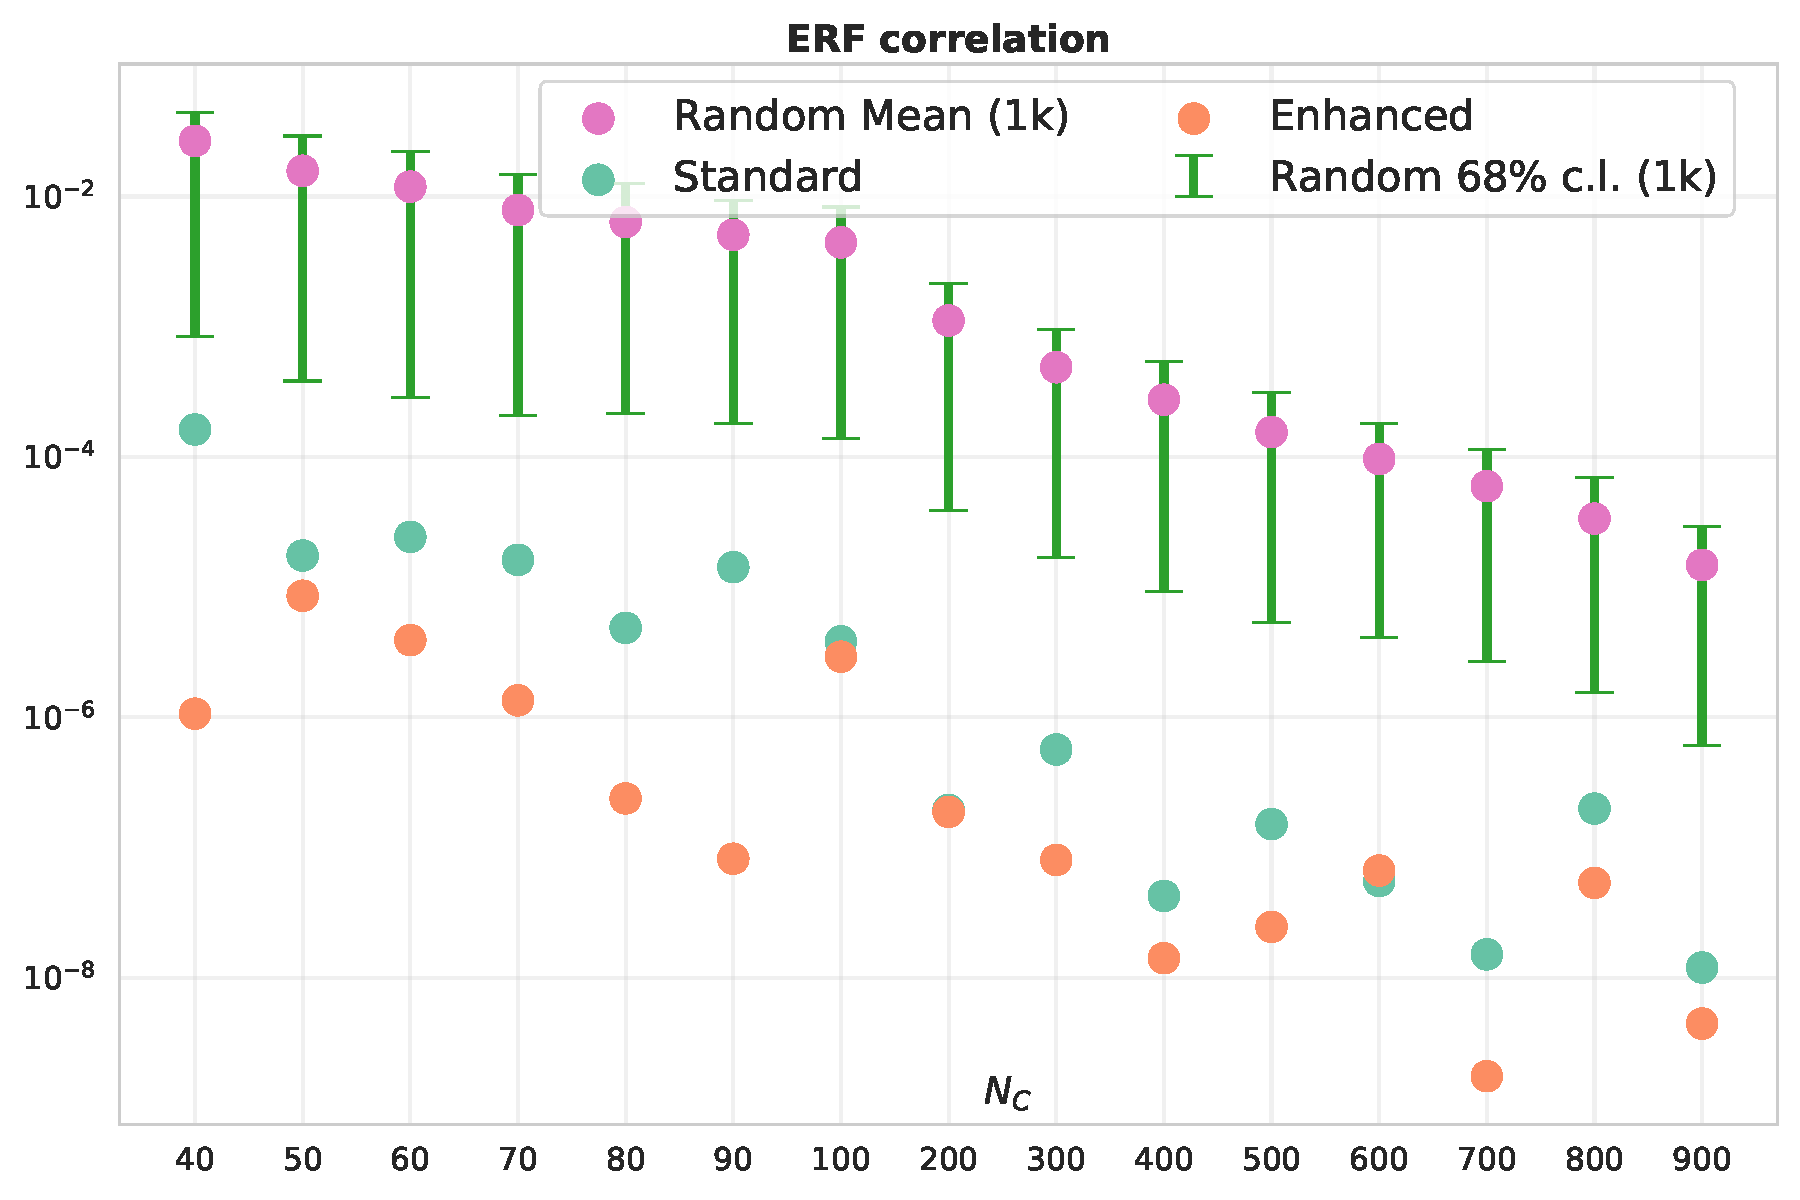
\includegraphics[width=\linewidth]{./gan_compressor/imgs/erf-validation.pdf}
	\end{column}
	\begin{column}{.5\textwidth}	
	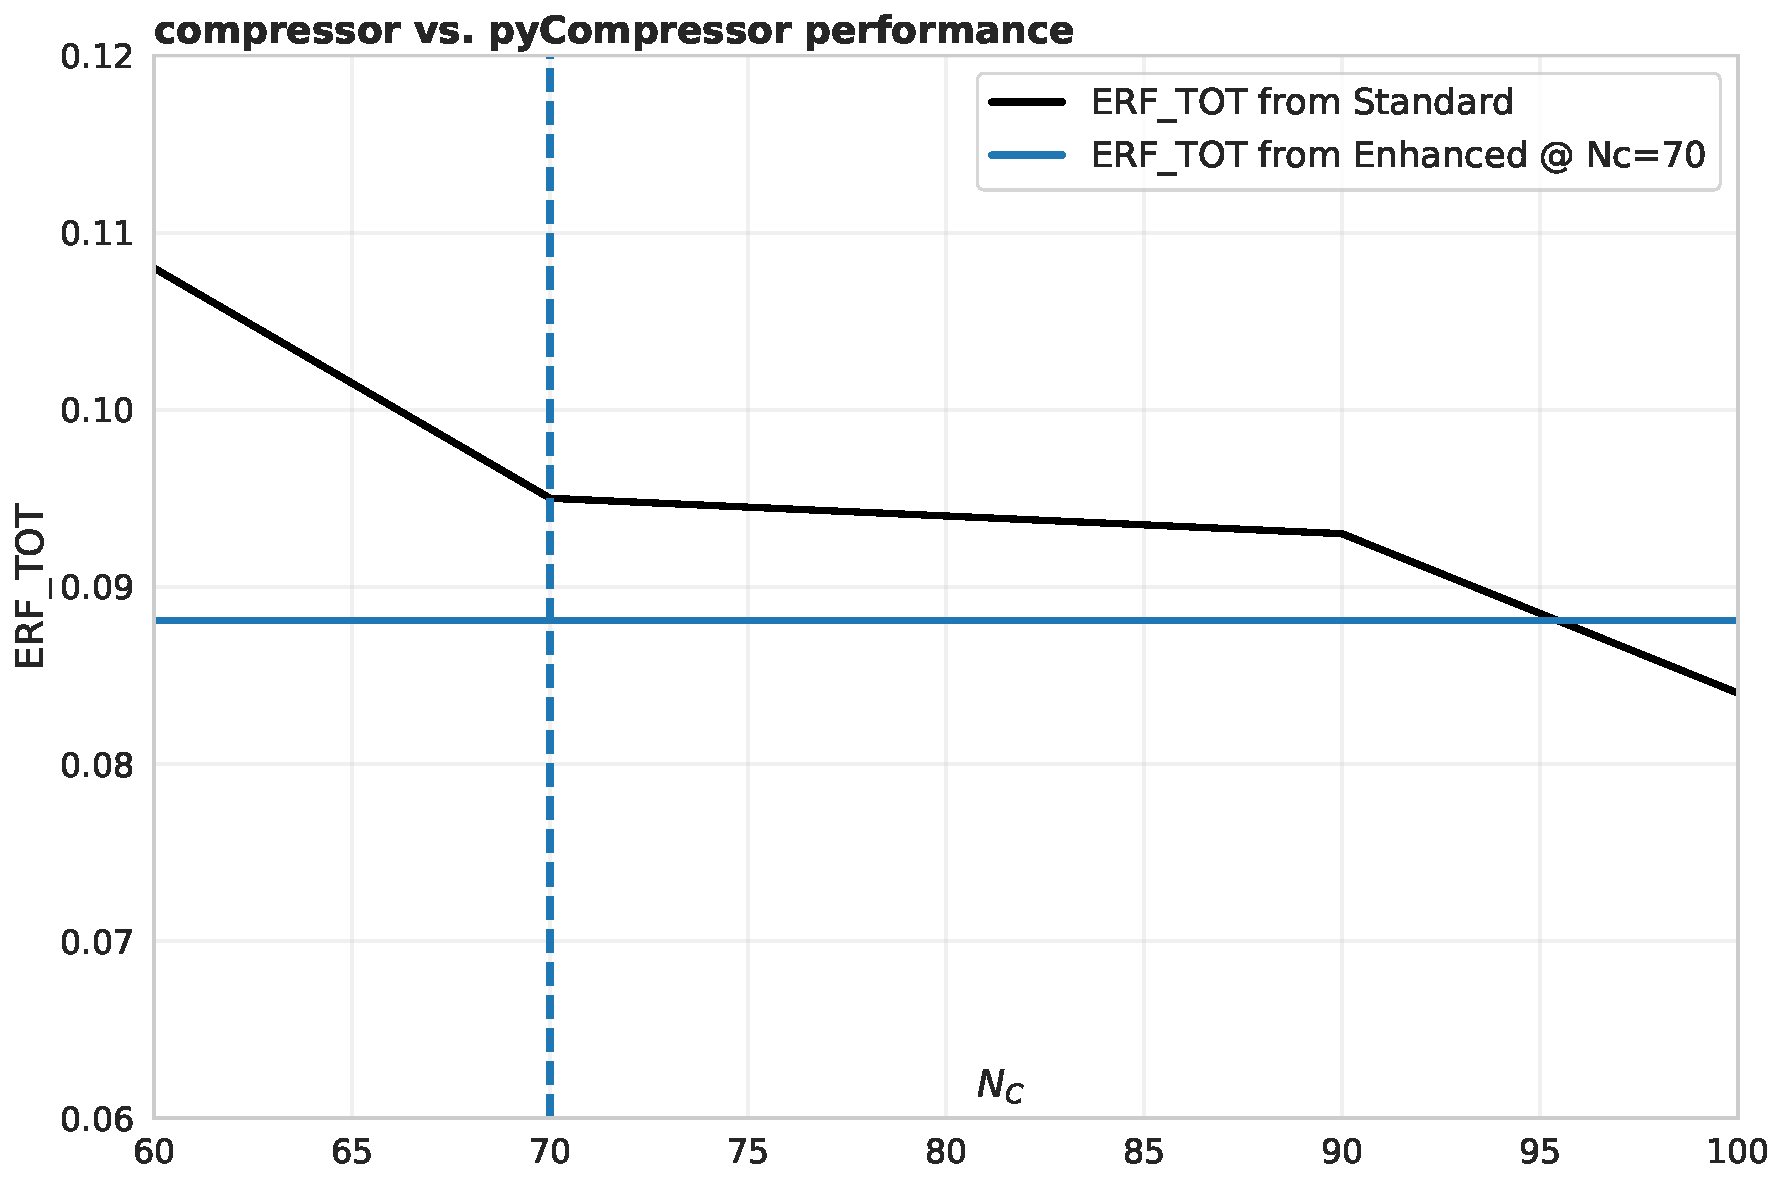
\includegraphics[width=\linewidth]{./gan_compressor/imgs/performance.pdf}
	\end{column}
	\end{columns}
	\begin{center}
	\begin{tcolorbox}[width=9.5cm, halign=center, colframe=HallowGreen]
		$N_c (\text{GAN-Enhanced})=70 \sim N_c (\text{Standard})=95$
	\end{tcolorbox}
	\end{center}
\end{frame}


%%%%%%%%%%%%%%%%%%%%%%%
\section{Additional slides}
\author[Christopher Schwan]{}
\institute{Universit\`a di Milano}

\subsection{Electroweak corrections}

\begin{frame}{EW corrections in PDF fits}
\fontsize{9}{11}\selectfont
\begin{equation*}
\colorbox{Goldenrod}{$\frac{\mathrm{d} \sigma_{ab}}{\mathrm{d} \mathcal{O}} (x_1, x_2, Q^2, \mathcal{O})$} = \sum_{m,n} \alpha_\mathrm{s}^m (Q^2) \alpha^n \colorbox{SkyBlue}{$\frac{\mathrm{d} \sigma_{ab}^{(m,n)}}{\mathrm{d} \mathcal{O}} (x_1, x_2, Q^2, \mathcal{O})$}
\end{equation*}
$\rightarrow$ \alert{only lowest order in $\alpha$ included in PDF fits}

\vspace*{\fill}

Known:
\begin{itemize}
\item LO QED ($+\text{N}^2\text{LO}$ QCD) PDFs are available (NNPDF, MMHT):
\begin{itemize}
\item non-zero photon PDF: LUXQED \beamercite{A.\ Manohar, P.\ Nason, G.\ P.\ Salam, G.\ Zanderighi}{https://inspirehep.net/literature/1475703},\\
\beamercite{A.\ Manohar, et al.}{https://inspirehep.net/literature/1614486}
\item lepton PDFs: LUXlep \beamercite{L.\ Buonocore, P.\ Nason, F.\ Tramontano, G.\ Zanderighi}{https://inspirehep.net/literature/1796368}
\item QED effects in the DGLAP equation
\end{itemize}
\item (some) QED effects subtracted in data
\end{itemize}

\vspace*{\fill}

Unknown:
\begin{itemize}
\item EW corrections are not (systematically) included in PDF fits; only NNLO QCD corrections
\item[$\rightarrow$] Inclusion of fully differential NLO EW corrections (no K factors) for \alert{all} PDF processes
\end{itemize}
\end{frame}

\begin{frame}{Why include NLO EW corrections?}
\fontsize{9}{11}\selectfont
\begin{itemize}
\item NNLO QCD+NLO EW more accurately than plain NNLO QCD
\item Do we need NLO EW corrections in PDF fits/Is LO QED enough?
\item[$\rightarrow$] Probably not now, but certainly in the future!
\item Already now: NNPDF cuts off a few observables because of large EW corrections\\
(e.g.\ $M_{\mathrm{e} \bar{\mathrm{e}}} \le \SI{210}{\giga\electronvolt}$ for the shown ATLAS measurement)
\end{itemize}
\vspace*{\fill}
\begin{block}{Programme: inclusion of NLO EW}
\begin{itemize}
\item allows \alert{inclusion} of observables with large EW corrections:\\
DY: large $M_{\ell \bar{\ell}}$, Z boson: large $p_\mathrm{T}$, \ldots
\item more \alert{accurate description} of observables: effects on PDFs?
\item[$\rightarrow$] systematic calculation of \alert{all} corrections (including QCD--EW), for \alert{all} processes\\
\enquote{the best PDFs demand the best predictions} as \alert{interpolation grids}
\item[$\rightarrow$] demands a more consistent data treatment, study \alert{double-counting} issues
\end{itemize}
\end{block}
\end{frame}

\begin{frame}{Interpolation grids (I)}
\fontsize{9}{11}\selectfont
For PDF fitting we need \alert{PDF independent} predictions. Use Lagrange interpolation,
\begin{equation*}
f_a (x_1, Q^2) f_b (x_2, Q^2) \approx \sum_{i,j,k} f_a ( x_i, Q^2_k ) f_b ( x_j, Q^2_k ) L_i (x_1) L_j (x_2) L_k (Q^2) \text{,}
\end{equation*}
with Lagrange polynomials $L_i$ over the 3D grid $\left\{ (x_i, x_j, Q^2_k) \right\}_{i,j,k}$. Insert into master formula:
\begin{equation*}
\begin{split}
\frac{\mathrm{d} \sigma}{\mathrm{d} \mathcal{O}} &= \sum_{a,b} \int_0^1 \mathrm{d} x_1 \int_0^1 \mathrm{d} x_2 \int_{Q^2_\text{min}}^{Q^2_\text{max}} \mathrm{d} Q^2 \, f_a (x_1, Q^2) f_b (x_2, Q^2) \colorbox{Goldenrod}{$\frac{\mathrm{d} \sigma_{ab}}{\mathrm{d} \mathcal{O}} (x_1, x_2, Q^2, \mathcal{O})$} \\
&= \sum_{a,b} \sum_{i,j,k} \sum_{m,n} f_a ( x_i, Q^2_k ) f_b ( x_j, Q^2_k ) \alpha_\mathrm{s}^m (Q^2) \alpha^n \colorbox{LimeGreen}{$\frac{\mathrm{d} \Sigma_{abijkmn}}{\mathrm{d} \mathcal{O}}$}
\end{split}
\end{equation*}
where
\begin{equation*}
\colorbox{LimeGreen}{$\frac{\mathrm{d} \Sigma_{abijkmn}}{\mathrm{d} \mathcal{O}}$} = \int_0^1 \mathrm{d} x_1 \int_0^1 \mathrm{d} x_2 \int_{Q^2_\text{min}}^{Q^2_\text{max}} \mathrm{d} Q^2 \, L_i (x_1) L_j (x_2) L_k (Q^2) \colorbox{SkyBlue}{$\frac{\mathrm{d} \sigma_{ab}^{(i,k)}}{\mathrm{d} \mathcal{O}} (x_1, x_2, Q^2, \mathcal{O})$}
\end{equation*}
$\rightarrow$ generate \colorbox{LimeGreen}{$\frac{\mathrm{d} \Sigma_{abijkmn}}{\mathrm{d} \mathcal{O}}$} \alert{once}, perform PDF convolutions very \alert{quickly off-line}
\end{frame}

\begin{frame}{Example: $\Sigma_{\mathrm{gg}ij021}/\Sigma_{\mathrm{gg}ij020}$, $\mathcal{O} (\alpha_\mathrm{s}^2 \alpha) / \mathcal{O} (\alpha_\mathrm{s}^2)$ for $\mathrm{g}\mathrm{g} \to \mathrm{t} \bar{\mathrm{t}}$ @ \SI{8}{\tera\electronvolt}}
\fontsize{9}{11}\selectfont
\begin{columns}[onlytextwidth]
\begin{column}{0.6\textwidth}
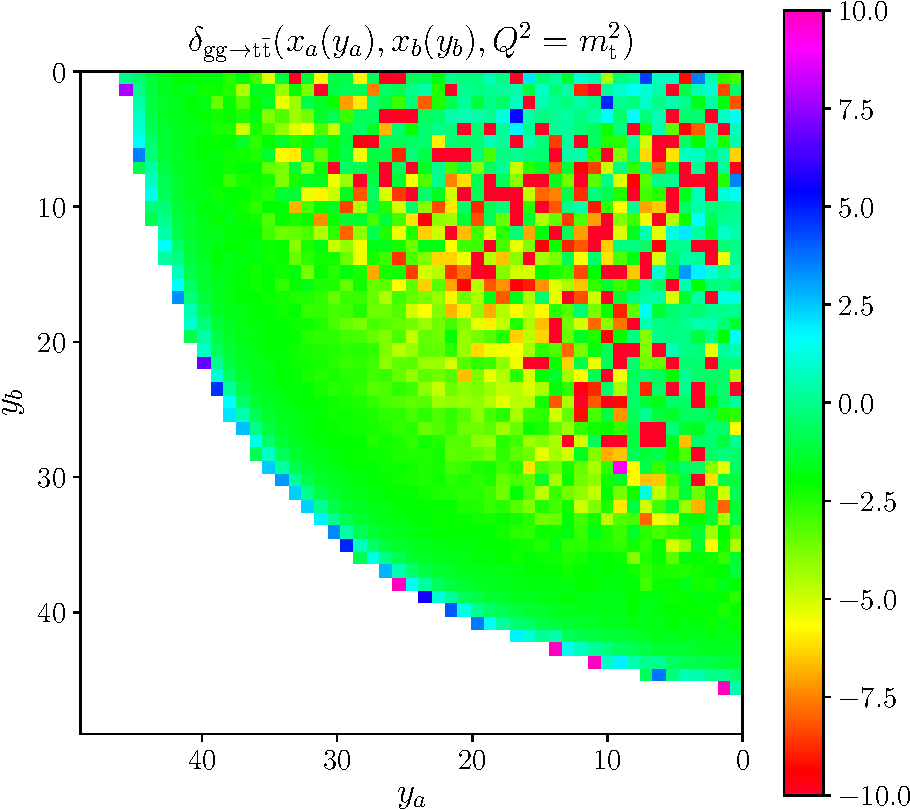
\includegraphics[height=0.73\textheight]{ew_corrections/figures/ttb-crop}
\end{column}
\begin{column}{0.4\textwidth}
\begin{itemize}
\item no interpolation in $y_a$, $y_b$, or $Q^2$
\item correction for ixs roughly \SI{-0.5}{\percent}
\item $y_{a/b}(x) = -\ln x_{a/b} + 5 (1-x_{a/b})$, $y(1) = 0$
\vspace*{0.25cm}
\item lower left corner $\rightarrow$ production threshold
\item at threshold: Coulomb singularity
\item $y_a \leftrightarrow y_b$ symmetry: initial-state symmetry of $\mathrm{g}\mathrm{g} \to \mathrm{t} \bar{\mathrm{t}}$
\item negative correction for larger $x_a$, $x_b$
\end{itemize}
\end{column}
\end{columns}
\end{frame}

\begin{frame}{Interpolation grids (II)}
\fontsize{9}{11}\selectfont
\begin{itemize}
\item Interpolation grids are an old idea:
\begin{itemize}
\item \textrm{\textsc{APPLgrid}} \beamercite{T.\ Carli et al.}{https://inspirehep.net/literature/837019}
\item \textrm{\textsc{fastNLO}} \beamercite{T.\ Kluge, K.\ Rabbertz, M.\ Wobisch}{https://inspirehep.net/literature/727193}
\end{itemize}
\item data generation with
\begin{itemize}
\item \textrm{\textsc{aMCfast}} \beamercite{V.\ Bertone, R.\ Frederix, S.\ Frixione, J.\ Rojo, M.\ Sutton}{https://inspirehep.net/literature/1303899} \\
(\textrm{\textsc{mg5\_aMC@NLO v2+APPLgrid}}) or
\item \textrm{\textsc{MCgrid}} \beamercite{L.D. Debbio, N.P.\ Hartland, S.\ Schuhmann}{https://inspirehep.net/literature/1269460} %\beamercite{E.\ Bothmann, N.P.\ Hartland, S.\ Schuhmann}{https://inspirehep.net/literature/1394617}
(\textrm{\textsc{SHERPA+APPLgrid/fastNLO}})
\item dedicated MCs: \textrm{\textsc{MCFM}}, \textrm{\textsc{NLOjet++}}
\end{itemize}
\item NNPDF uses \textrm{\textsc{APPLgrid}}
\item None of the above support EW corrections
\item \textrm{\textsc{APPLgrid}} is slow and difficult to use; \textrm{\textsc{fastNLO}} has complicated interface
\end{itemize}

\vspace*{\fill}

\begin{itemize}
\item[$\rightarrow$] We wrote \textrm{\textsc{PineAPPL}} (\textrm{\textsc{PineAPPL}} Is Not an Extension of \textrm{\textsc{APPLgrid}})
\item supports arbitrary fixed-order calculations
\item easily supports distributions with more than 1000 bins
\item interfacing with
\begin{itemize}
\item \textrm{\textsc{mg5\_aMC@NLO v3.0.4}} complete, will be released soon
\item \textrm{\textsc{SHERPA+MCgrid}} in progress
\item your custom MC (should be) easily possible!
\end{itemize}
\end{itemize}
\end{frame}

\begin{frame}{\textrm{\textsc{PineAPPL}}}
\fontsize{9}{11}\selectfont
\begin{columns}[T,onlytextwidth]
\begin{column}{.5\textwidth}
\begin{itemize}
\item \beamercite{S.\ Carazza, E.R.\ Nocera, C.\ Schwan, M.\ Zaro}{https://inspirehep.net/literature/1814432}
\item interpolation error typically sub-per mille (see right)
\item off-line PDF uncertainty calculation in a few seconds
\item command-line program to quickly produce predictions
\item simply add: \texttt{set pineappl True} to \texttt{mg5\_aMC} runcard
\item \texttt{C}, \texttt{Python}, \texttt{Rust} interfaces available
\item size of each order, partonic channels, observable
\item support for 1D, 2D, 3D, \ldots, nD distributions
\end{itemize}

\vspace*{0.5cm}

\url{https://n3pdf.github.io/pineappl}
\end{column}
\begin{column}{.5\textwidth}
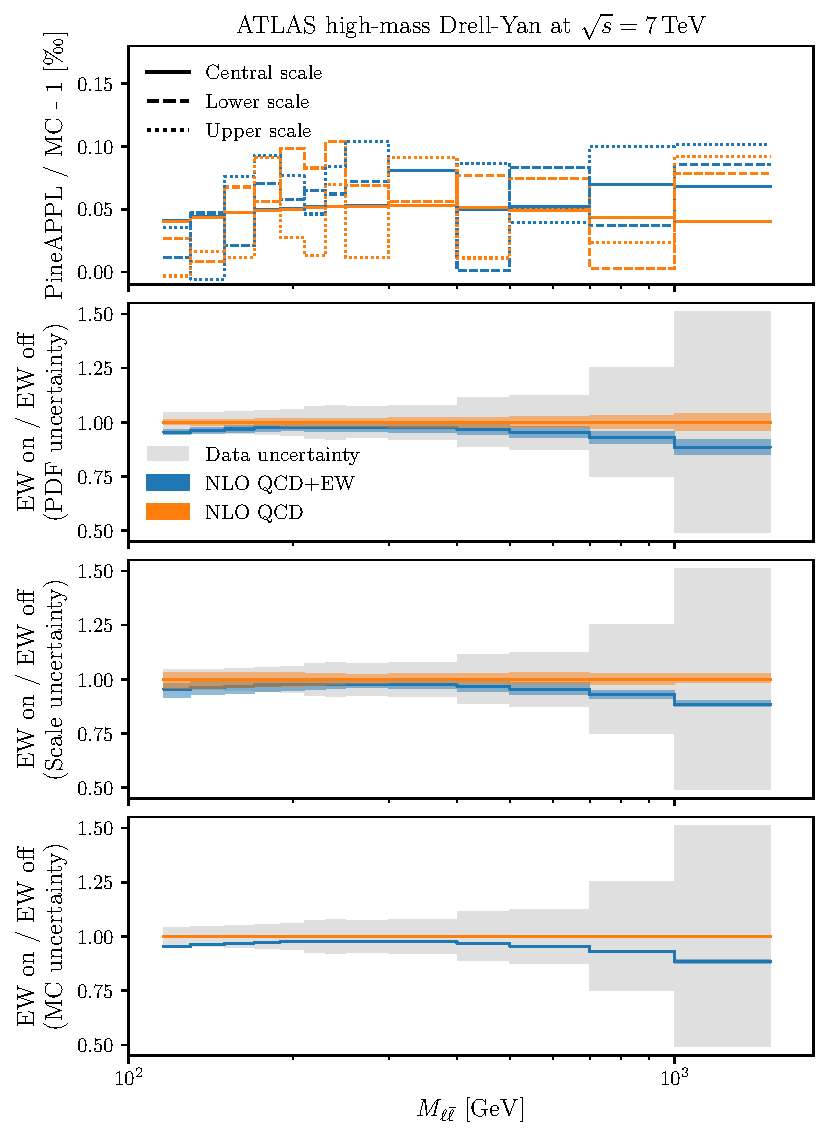
\includegraphics[height=0.89\textheight]{ew_corrections/figures/pineappl_ATLASZHIGHMASS49FB}
\end{column}
\end{columns}
\end{frame}

\begin{frame}{Process list for NNPDF4.0}
\fontsize{9}{11}\selectfont
Calculate theoretical predictions for the entire NNPDF4.0 dataset:
\begin{enumerate}
\item DIS: NMC, SLAC, BCDMS, CHORUS, NUTEV, HERA
\item Fixed-target Drell--Yan experiments
\item Collider experiments (CDF, D{\O}, ATLAS, and CMS)
\begin{itemize}
\item Drell--Yan $\mathrm{Z}$ and $\mathrm{W}^\pm$
\item dijets ATLAS \SI{7}{\tera\electronvolt} and CMS \SIlist{7;8}{\tera\electronvolt} (NEW)
\item single-inclusive jet production ATLAS \SI{8}{\tera\electronvolt} (NEW); peculiar observable,\\
see \beamercite{M.\ Cacciari, S.\ Forte, D.\ Napoletano, G.\ Soyez, G.\ Stagnitto}{https://inspirehep.net/literature/1741988}
\item Top-pair production
\item Z transverse momentum
\item $\mathrm{W}^\pm + \mathrm{c}$ production (at NLO only)
\item W + jets (NEW)
\item single top t-channel production (NEW)
\item diphoton production (NEW)
\end{itemize}
\end{enumerate}

\vspace*{\fill}

\begin{itemize}
\item[$\rightarrow$] for the time being \alert{only collider experiments}; ($N_\text{dat} \approx 1200$)\\
\item[$\rightarrow$] write runcards, validate\\
\item[$\rightarrow$] \alert{explore double-counting issues}, problems with data
\end{itemize}
\end{frame}

\begin{frame}{Drell--Yan: NNPDF4.0 dataset}
\fontsize{9}{11}\selectfont
\begin{columns}[T,onlytextwidth]
\begin{column}{.5\textwidth}

\centering
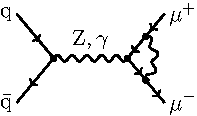
\includegraphics[width=0.32\textwidth]{ew_corrections/figures/fd04_loop_vertex_correction}
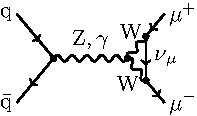
\includegraphics[width=0.32\textwidth]{ew_corrections/figures/fd07_loop_vertex_w_bosons}
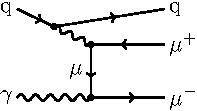
\includegraphics[width=0.32\textwidth]{ew_corrections/figures/fd06_photon_quark_real}

\vspace*{0.4cm}


{\tiny
\begin{center}
\begin{tabular}{@{}l@{~}r@{~}|@{~}l@{~}r@{}}
\toprule
NNPDF ID & $\sqrt{s}$ & NNPDF ID & $\sqrt{s}$ \\
\midrule
\texttt{CDFZRAP} & \SI{1.96}{\tera\electronvolt} & 
\texttt{CMSWEASY840PB} & \SI{7}{\tera\electronvolt} \\
\texttt{D0ZRAP} & \SI{1.96}{\tera\electronvolt} & 
\texttt{CMSWMASY47FB} & \SI{7}{\tera\electronvolt} \\
\texttt{D0WMASY} & \SI{1.96}{\tera\electronvolt} & 
\alert{\texttt{CMSDY2D11}} & \alert{\SI{7}{\tera\electronvolt}} \\
\texttt{ATLASWZRAP36PB} & \SI{7}{\tera\electronvolt} & 
\texttt{CMSWMU8TEV} & \SI{8}{\tera\electronvolt} \\
\texttt{ATLASZHIGHMASS49FB} & \SI{7}{\tera\electronvolt} & 
\texttt{LHCBZ940PB} & \SI{7}{\tera\electronvolt} \\
\texttt{ATLASLOMASSDY11EXT} & \SI{7}{\tera\electronvolt} & 
\texttt{LHCBZEE2FB} & \SI{8}{\tera\electronvolt} \\
\texttt{ATLASWZRAP11CC} & \SI{7}{\tera\electronvolt} & 
\texttt{LHCBWZMU7TEV} & \SI{7}{\tera\electronvolt} \\
\texttt{ATLASWZRAP11CF} & \SI{7}{\tera\electronvolt} & 
\texttt{LHCBWZMU8TEV} & \SI{8}{\tera\electronvolt} \\
\texttt{ATLAS\_DY2D\_8TEV} & \SI{8}{\tera\electronvolt} & 
\texttt{LHCB\_Z\_13TEV\_DIMUON} & \SI{13}{\tera\electronvolt} \\
\texttt{ATLAS\_WZ\_TOT\_13TEV} & \SI{13}{\tera\electronvolt} & 
\texttt{LHCB\_Z\_13TEV\_DIELECTRON} & \SI{13}{\tera\electronvolt} \\
\bottomrule
\end{tabular}
\end{center}
}

\begin{itemize}
\item Observables:
$y_{\ell \bar{\ell}} \approx \frac{1}{2} ln \frac{x_1}{x_2}$ and $M_{\ell \bar{\ell}} \approx \sqrt{x_1 x_2 s}$
\item analysis: \beamercite{CMS Collaboration}{https://inspirehep.net/literature/1262319}
\item NLO EW / NLO QCD: \SI{+11}{\percent} correction, coming from FSR
\end{itemize}

\end{column}
\begin{column}{.5\textwidth}
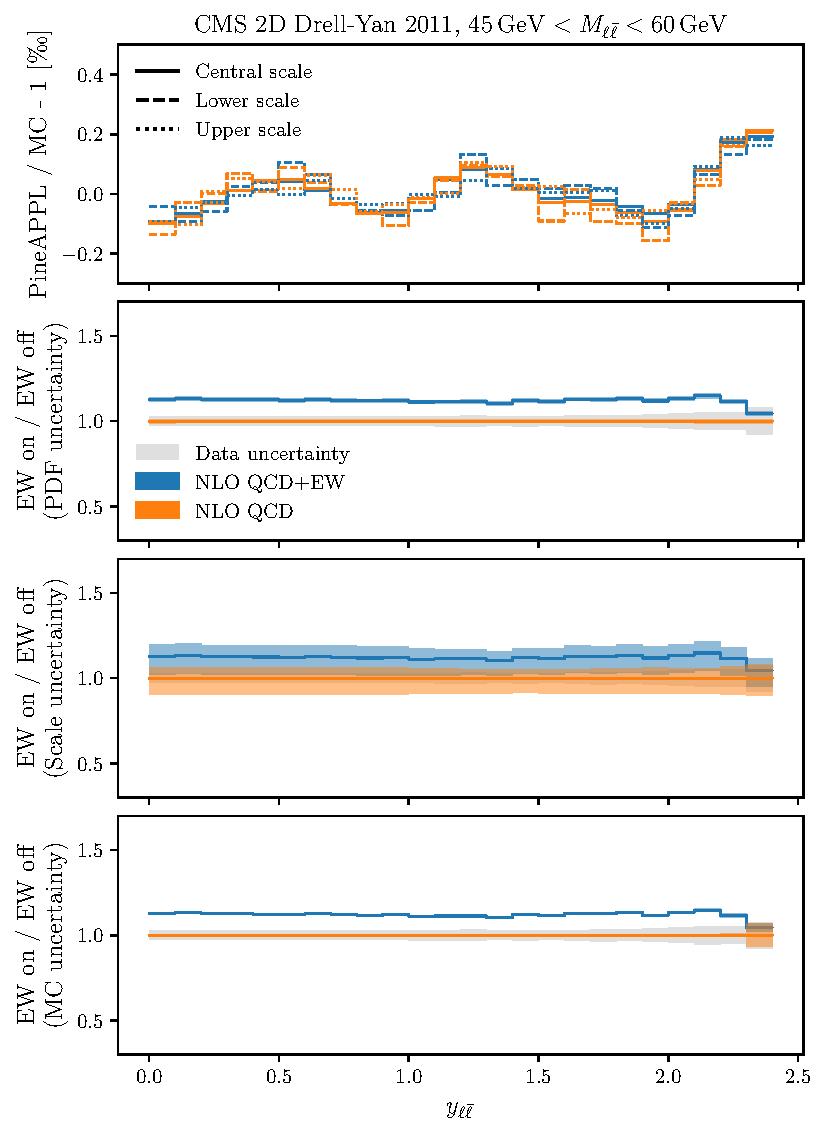
\includegraphics[width=0.94\textwidth]{ew_corrections/figures/pineappl_CMSDY2D11_bin3}
\end{column}
\end{columns}
\end{frame}

\begin{frame}{Double-counting problem: subtraction of FSR}
\fontsize{9}{11}\selectfont
\begin{center}
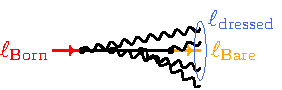
\includegraphics[height=0.2\textheight]{ew_corrections/figures/fd05_photon_radiation}
\end{center}
\begin{itemize}
\item \textcolor{red}{pre-FSR data/Born leptons}: observables of leptons \enquote{before they radiate}, calculated using photon-shower inversion (\textrm{\textsc{PHOTOS}}), from
\item \textcolor{RoyalBlue}{post-FSR data/dressed leptons}: observables using leptons with photons recombined around $\Delta R_{f \gamma}$, typically $\Delta R_{f \gamma} = 0.1$
\end{itemize}
\begin{itemize}
\item \textcolor{red}{pre-FSR data} for comparisons with \textcolor{red}{QCD}-only theory predictions
\item \textcolor{RoyalBlue}{post-FSR data} for comparisons with \textcolor{RoyalBlue}{EW} corrections (up to one photon emission)
\end{itemize}

\vspace*{\fill}

\begin{itemize}
\item Some experiments---notably CMS---do not publish post-FSR data: double counting issue!
\item dressing factors
\begin{equation*}
C_\text{dress} = \frac{\mathrm{d} \sigma_\text{post-FSR} / \mathrm{d} \mathcal{O}}{\mathrm{d} \sigma_\text{pre-FSR} / \mathrm{d} \mathcal{O}}
\end{equation*}
can be large, \alert{up to \SI{20}{\percent}} in invariant mass distributions
\item Often $C_\text{dress}$ (+uncertainty) and pre-FSR dataset given $\Rightarrow$ need to change systematic uncertainties!
\end{itemize}
\end{frame}

\begin{frame}{Subtraction of photon--photon contribution}
\fontsize{9}{11}\selectfont
\begin{center}
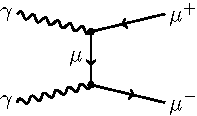
\includegraphics[height=0.2\textheight]{ew_corrections/figures/fd02_born_photon_t_channel}
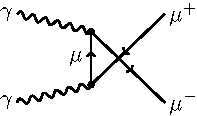
\includegraphics[height=0.2\textheight]{ew_corrections/figures/fd03_born_photon_u_channel}
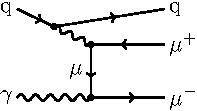
\includegraphics[height=0.2\textheight]{ew_corrections/figures/fd06_photon_quark_real}
\end{center}
\vspace*{\fill}
\begin{itemize}
\item For ATLAS and CMS it seems to be standard procedure to subtract double-photon induced contributions:
\begin{displayquote}
The photon-induced process, $\gamma\gamma \to \ell \bar{\ell}$, is simulated at LO using Pythia 8 and the MRST2004qed PDF set.
\end{displayquote}
\item I am not sure why this is done
\item This is a problem: proton contains photons, should be counted towards signal!
\item Size of the LO contribution can become significant in large-invariant-mass bins (\SI{3}{\percent}) depending on the used PDF---up to twice as large for pre-LUXQED photon PDFs
\end{itemize}
\end{frame}

\begin{frame}[t]{Z transverse momentum}
\fontsize{9}{11}\selectfont
\begin{columns}[T,onlytextwidth]
\begin{column}{.5\textwidth}
\hspace*{1.5cm}
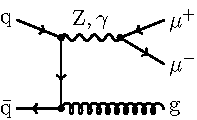
\includegraphics[height=0.13\textheight]{ew_corrections/figures/fd08_z_pt_born}

\vspace*{0.2cm}

\begin{center}
\alert<1>{$\mu = M_\mathrm{Z}$} vs.\ \alert<2>{$\mu = \sqrt{M_\mathrm{Z}^2 + (p_\mathrm{T}^{\ell \bar{\ell}})^2}$}
\end{center}
%\texttt{ATLASZPT8TEVMDIST}
%\texttt{ATLASZPT8TEVYDIST}
%\texttt{ATLAS\_WP\_JET\_8TEV\_PT}
%\texttt{ATLAS\_WM\_JET\_8TEV\_PT}
%\texttt{CMSZDIFF12}
\begin{itemize}
\item FSR issues similar to DY
\item no photon subtraction
\end{itemize}
static scale:
\begin{itemize}
\item accidental cancellation of NLO QCD correction $\rightarrow$ uncertainty band shrinks
\item NLO EW are artificially enhanced because of normalisation
\end{itemize}
dynamic scale:
\begin{itemize}
\item scale variation is stabilised
\item still significant EW corrections, comparable to data uncertainty
\end{itemize}
\end{column}
\begin{column}{.5\textwidth}
\only<1>{\hspace*{\fill}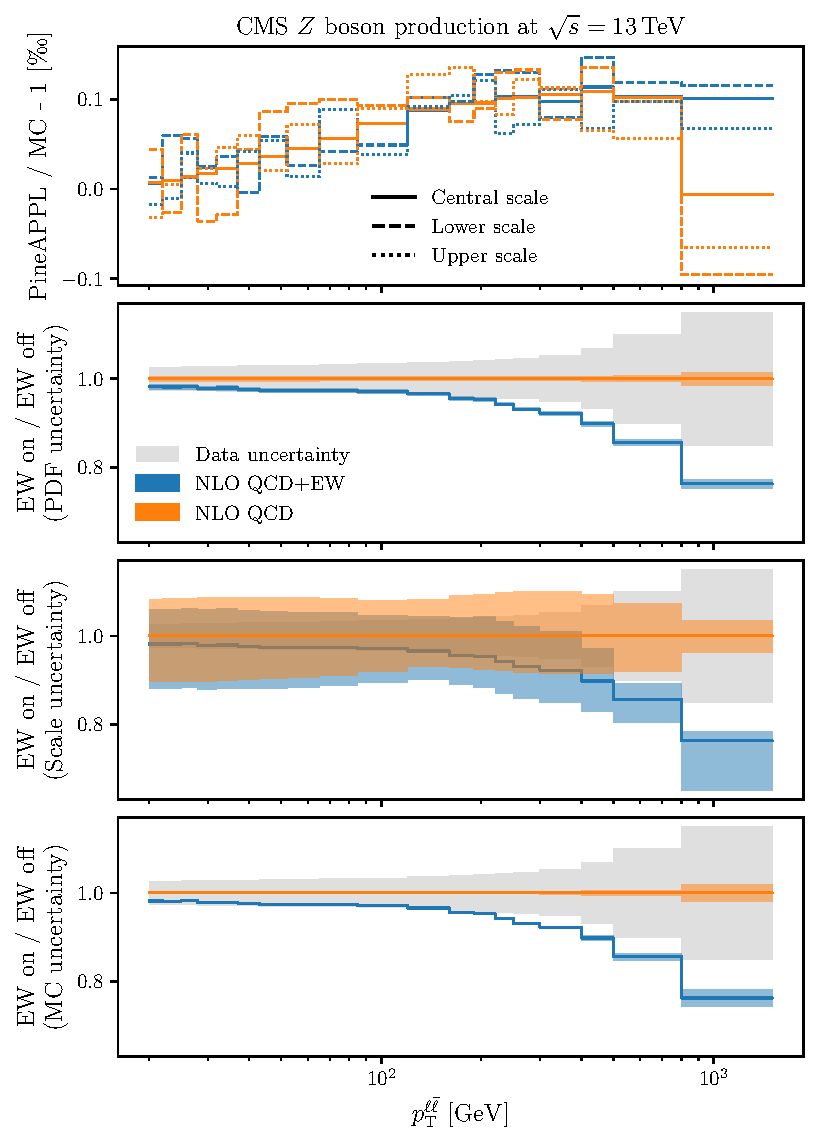
\includegraphics[width=0.9\textwidth]{ew_corrections/figures/pineappl_CMS_Z_13_TEV}}
\only<2>{\hspace*{\fill}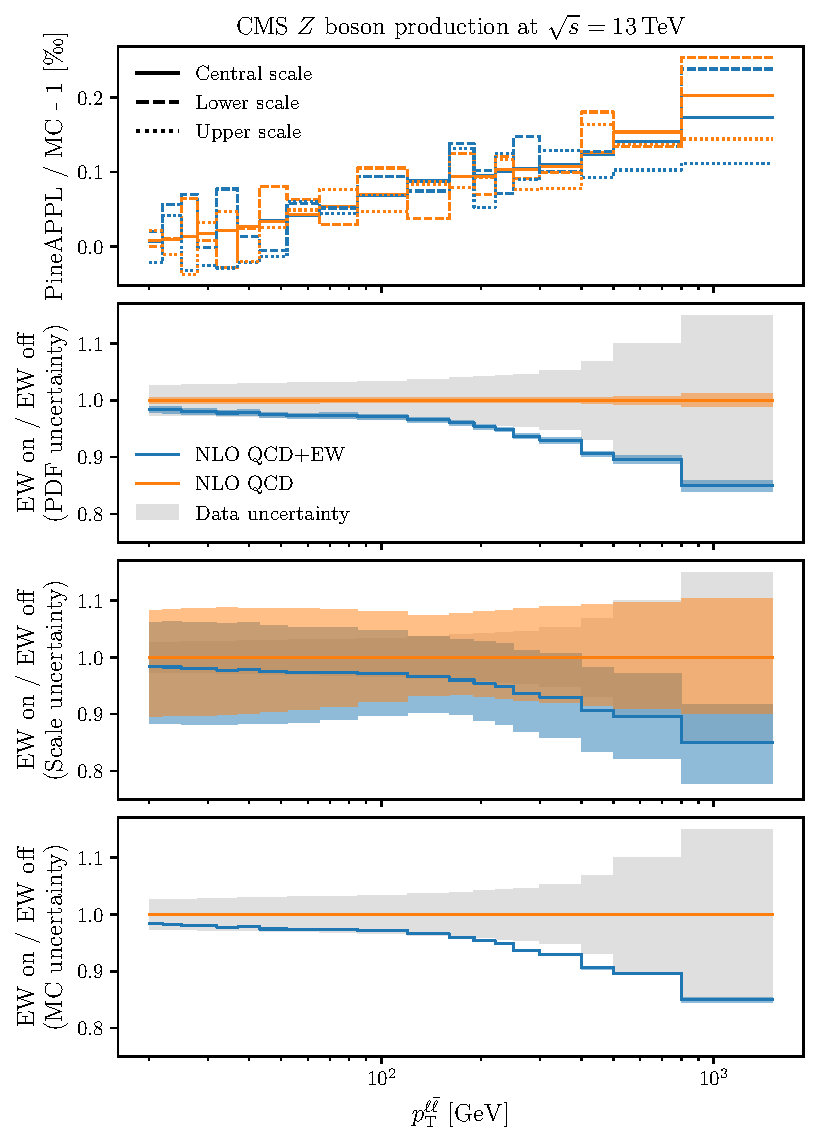
\includegraphics[width=0.9\textwidth]{ew_corrections/figures/pineappl_CMS_Z_13_TEV_dyn}}
\end{column}
\end{columns}
\end{frame}

\begin{frame}{Single-top production}
\fontsize{9}{11}\selectfont
Not properly definable (!?) at NLO EW:
\begin{itemize}
\item Analyses, e.g.\ \beamercite{ATLAS collaboration}{https://inspirehep.net/literature/1303905}, treat $s$-channels as background
\item single-production at LO:
\begin{center}
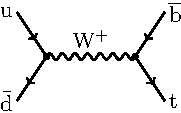
\includegraphics{ew_corrections/figures/fd10_born_s_channel_top}\hspace{0.4cm}
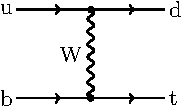
\includegraphics{ew_corrections/figures/fd11_born_t_channel_top}
\end{center}
\item but at NLO EW not (gauge-invariantly) separable:
\begin{center}
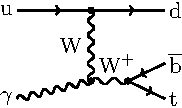
\includegraphics{ew_corrections/figures/fd12_real_ts_channel_top}\hspace{0.4cm}
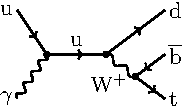
\includegraphics{ew_corrections/figures/fd13_real_s_channel_top}
\end{center}
\item[$\rightarrow$] ignore these datasets?
\item probably not too important, but see \beamercite{E.R.\ Nocera, M.\ Ubiali, C.\ Voisey}{https://inspirehep.net/literature/1772052}
\end{itemize}
\end{frame}

\begin{frame}{\href{https://arxiv.org/abs/1412.1115}{CMS DY 2D} (I)}
\fontsize{9}{11}\selectfont
\begin{columns}
\begin{column}{0.5\textwidth}
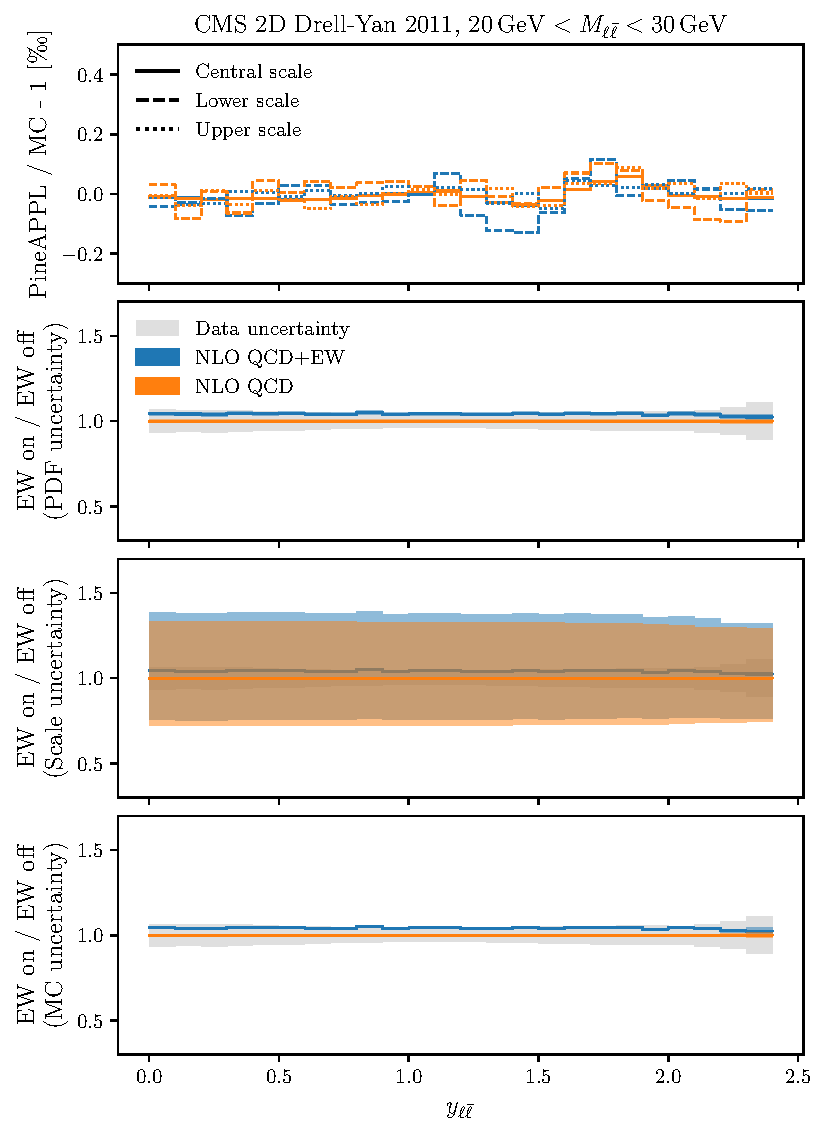
\includegraphics[width=0.95\textwidth]{ew_corrections/figures/pineappl_CMSDY2D11_bin1}
\end{column}
\begin{column}{0.5\textwidth}
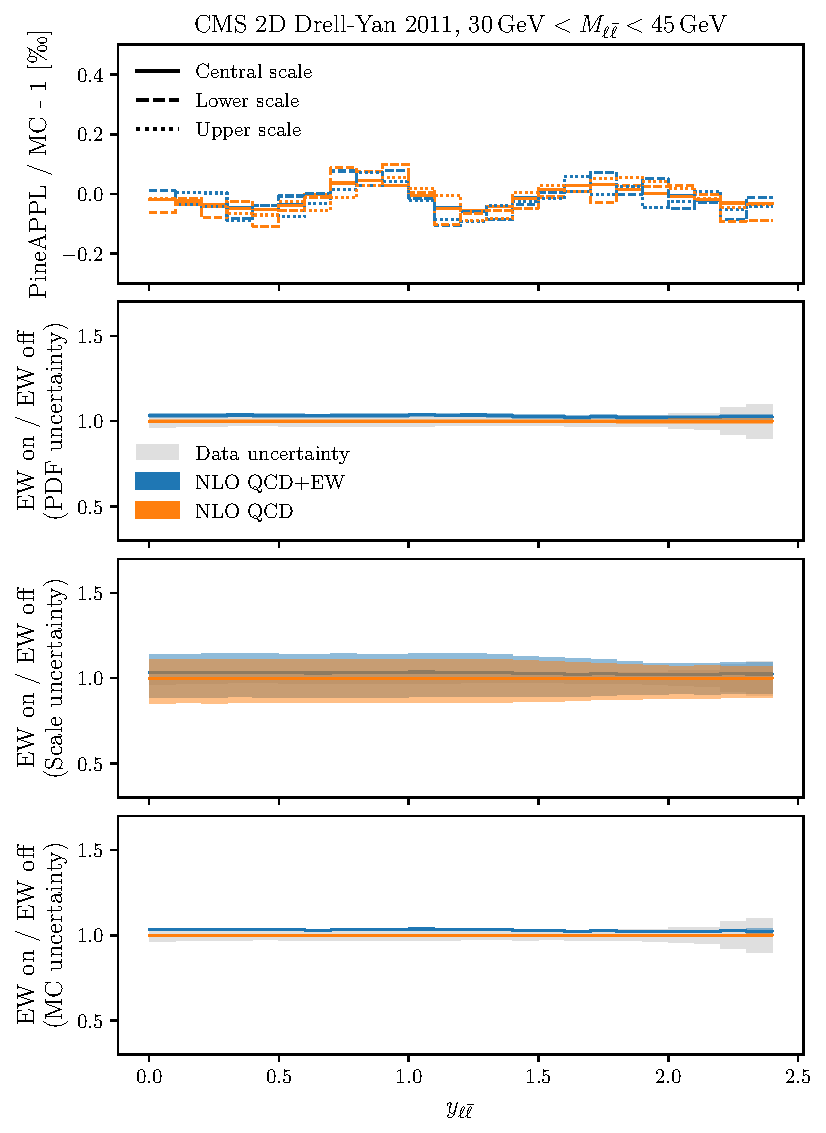
\includegraphics[width=0.95\textwidth]{ew_corrections/figures/pineappl_CMSDY2D11_bin2}
\end{column}
\end{columns}
\end{frame}

\begin{frame}{\href{https://arxiv.org/abs/1412.1115}{CMS DY 2D} (II)}
\fontsize{9}{11}\selectfont
\begin{columns}
\begin{column}{0.5\textwidth}
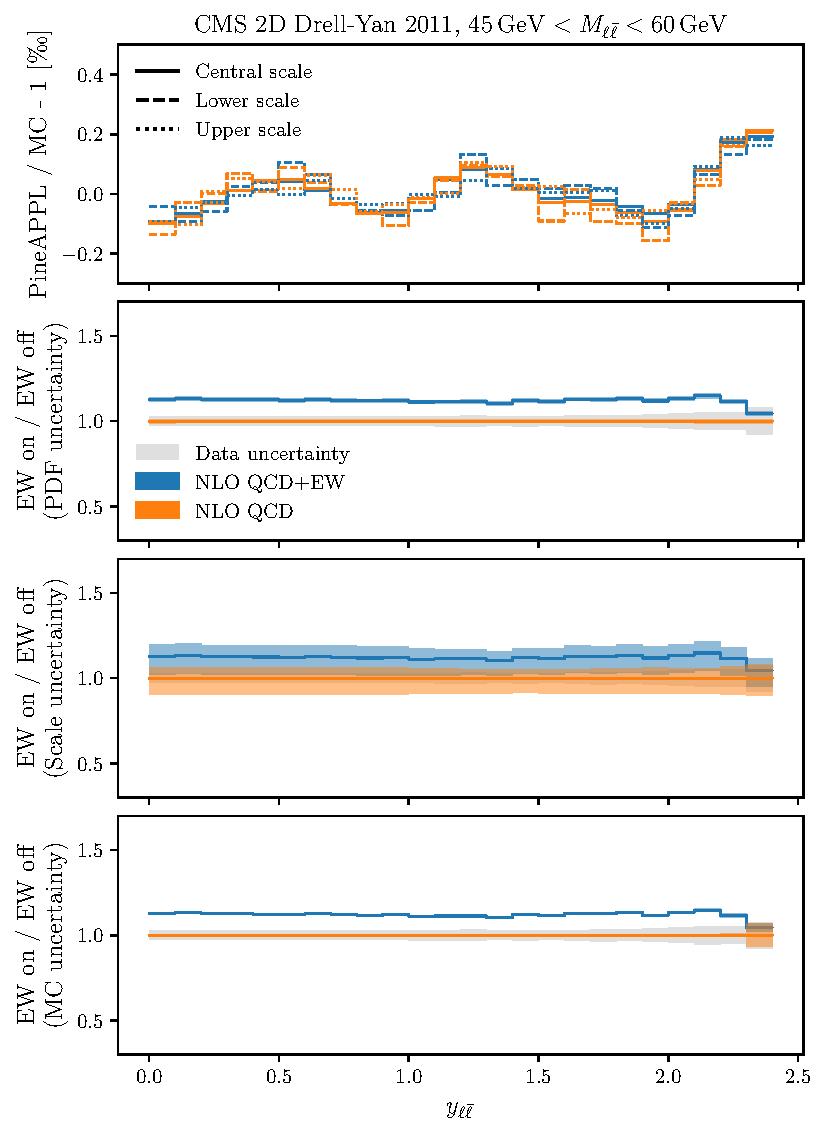
\includegraphics[width=0.95\textwidth]{ew_corrections/figures/pineappl_CMSDY2D11_bin3}
\end{column}
\begin{column}{0.5\textwidth}
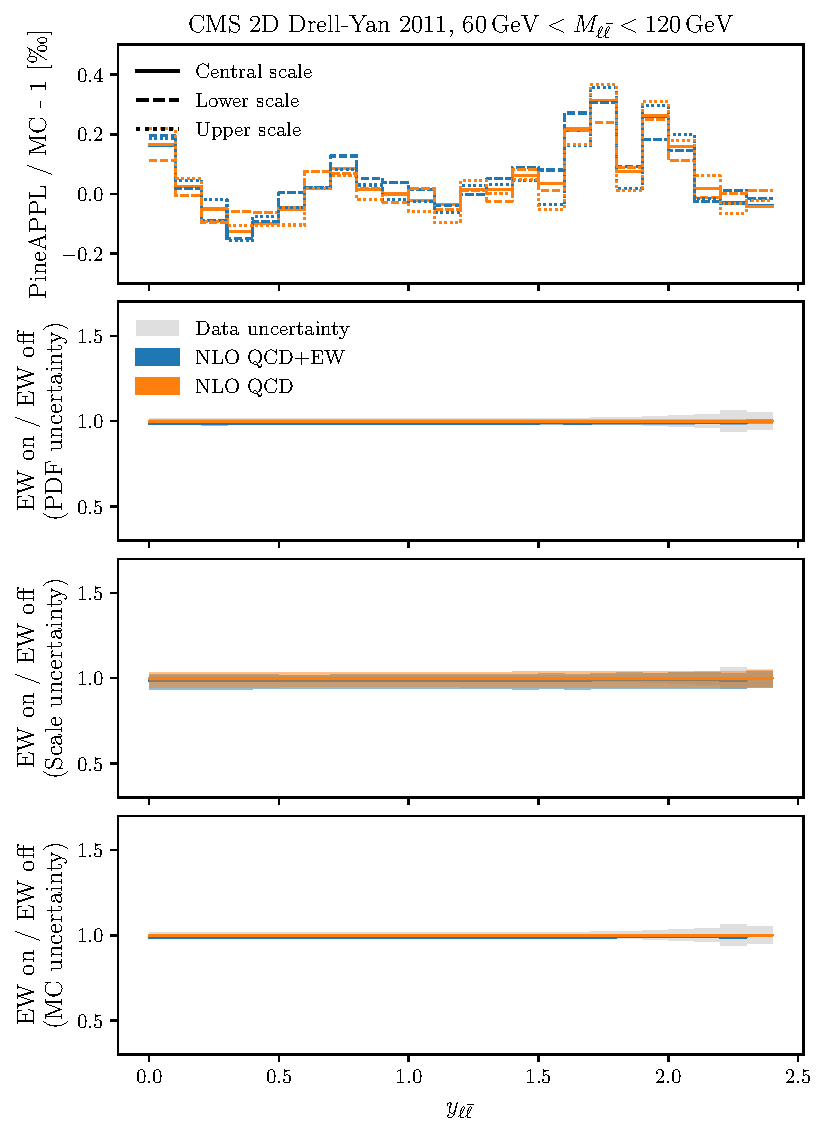
\includegraphics[width=0.95\textwidth]{ew_corrections/figures/pineappl_CMSDY2D11_bin4}
\end{column}
\end{columns}
\end{frame}

\begin{frame}{\href{https://arxiv.org/abs/1412.1115}{CMS DY 2D} (III)}
\fontsize{9}{11}\selectfont
\begin{columns}
\begin{column}{0.5\textwidth}
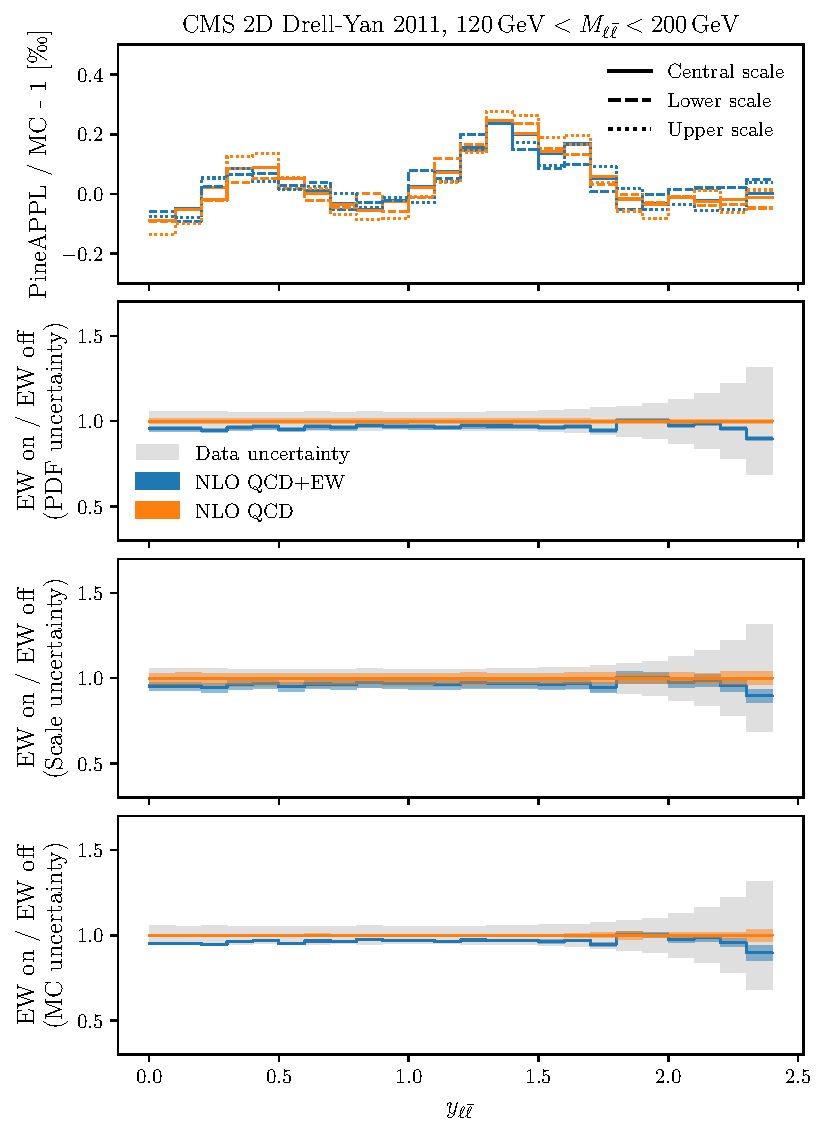
\includegraphics[width=0.95\textwidth]{ew_corrections/figures/pineappl_CMSDY2D11_bin5}
\end{column}
\begin{column}{0.5\textwidth}
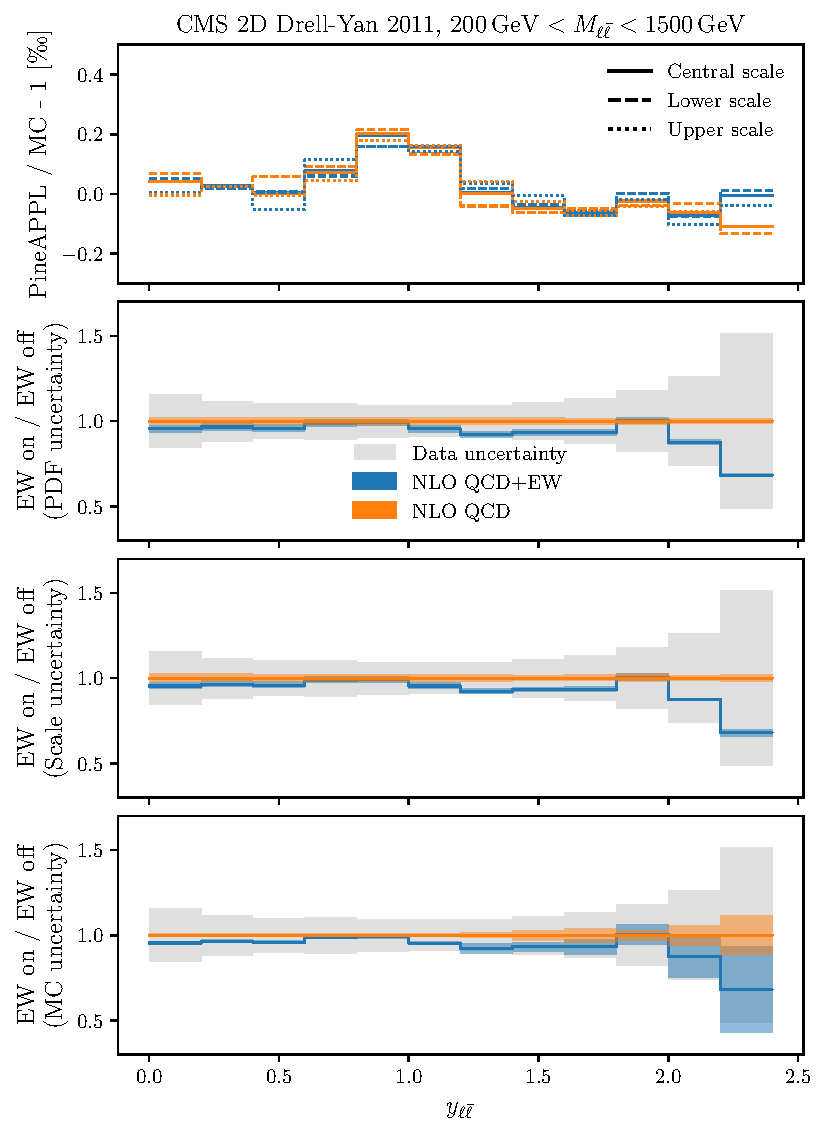
\includegraphics[width=0.95\textwidth]{ew_corrections/figures/pineappl_CMSDY2D11_bin6}
\end{column}
\end{columns}
\end{frame}

\author[Rosalyn Pearson]{}
\institute{University of Edinburgh}
\subsection{Deuteron and nuclear uncertainties}
\begin{frame}{Extra: Nuclear and deuteron observables}
\footnotesize{Deuteron (top) and heavy nuclear (bottom) }
  \begin{figure}
    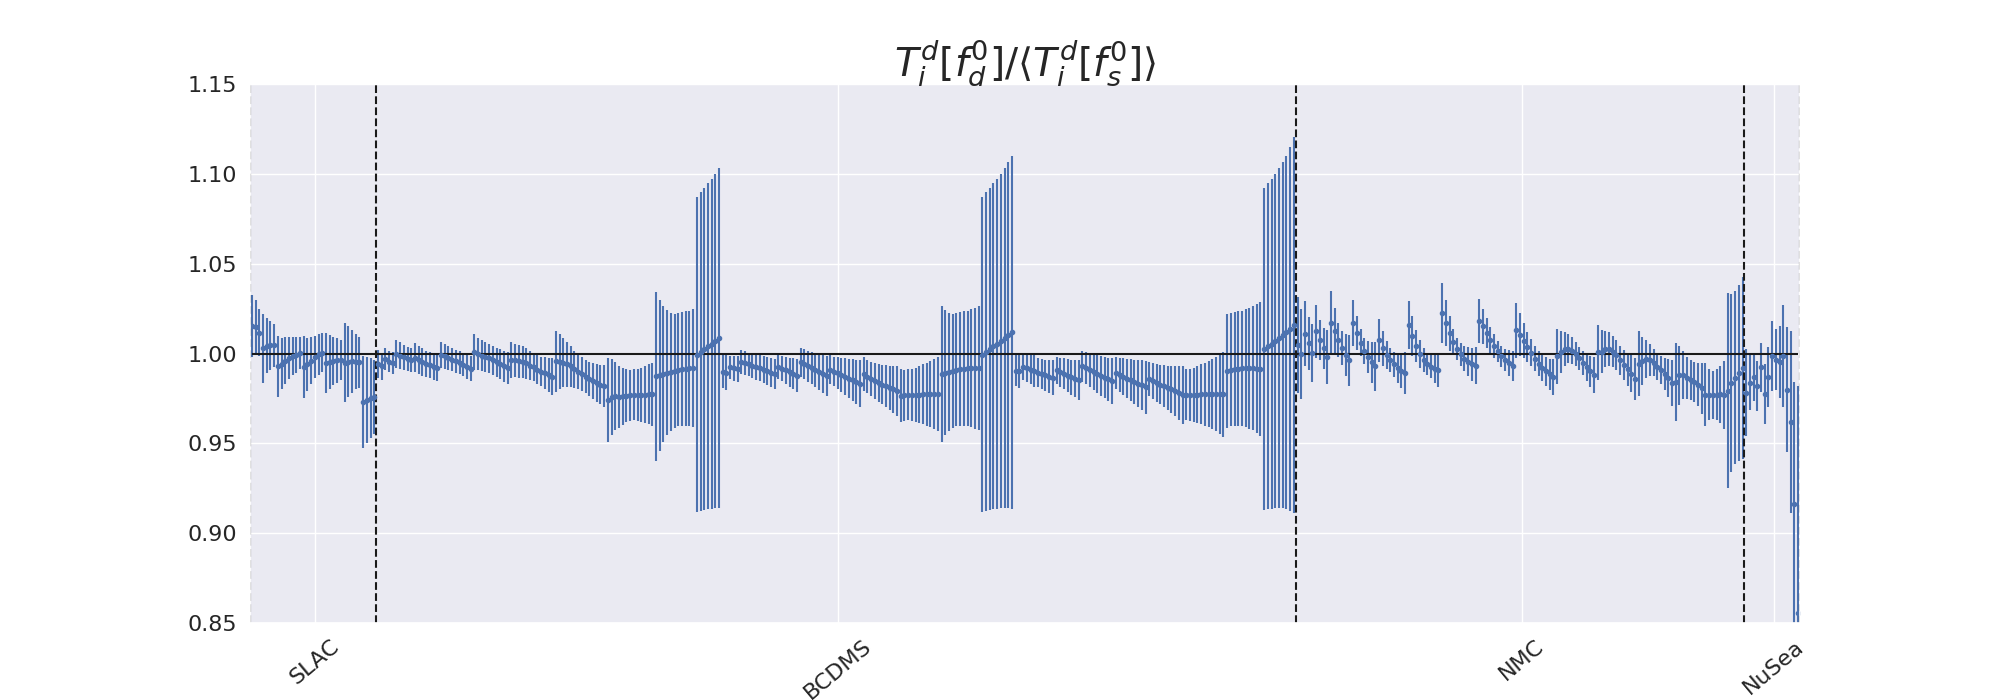
\includegraphics[width=90mm, trim={30mm, 0, 30mm, 0}]{nuclear_uncs/obsdeut.png}
    \includegraphics[width=85mm]{nuclear_uncs/obsnuc.png}
  \end{figure}
\end{frame}

\begin{frame}{Extra: deuteron uncertainties}

\begin{block}{Deuteron data}
{\bf Deuteron only} $F_2^d$: SLAC, BCDMS  $\to T_i^d[f_d]$
\newline
{\bf Mixed} $F_2^d/F_2^p$ \& $\sigma_{pd}^{DY}/\sigma_{pp}^{DY}$: NMC, DYE866/NuSea  $ \to T_i^d[f_d, f_p]$
\end{block}
Standard is to use isoscalar PDFs in place of deuteron: $f_s \equiv \frac{1}{2}(f_p + f_d)$
Now 
\begin{equation}
\Delta_i^{(k)} = \begin{cases}
T_i^d[f_d^{(k)}] - T_i^d[f_s^{(0)}] & i \in \text{deuteron only}\\
T_i^d[f_d^{(k)}, f_p^{(0)}] - T_i^d[f_s^{(0)}, f_p^{(0)}] & i \in \text{mixed}
\end{cases}
\end{equation}
\end{frame}

\begin{frame}{Extra: heavy nuclear uncertainties}

\begin{block}{Heavy nuclear data $T_i^N[f_N]$}
{\bf Cu}: DYE605,  $N=64$
\newline
{\bf Fe}: NuTeV (\& EMC), $N=56$
\newline
{\bf Pb}: CHORUS, $N=208$
\end{block}
\begin{equation}
\Delta_i^{(k)} = T_i^{N}[f_{N}^{(k)}] - T_i^{N}[f_{p}]
\end{equation}
Where 
\begin{equation}
\begin{split}
    T_i^N[f_N] = \frac{1}{A} (ZT_i[f_{p/N} + (A-Z)T_i[f_{n/N}] \\
    T_i^N[f_p] = \frac{1}{A} (ZT_i[f_p] +  (A-Z)T_i[f_n]
\end{split}
\end{equation}
\end{frame}
\begin{frame}{Extra: Correlation matrix}
  \begin{figure}
  \centering
    \includegraphics[width=40mm]{nuclear_uncs/covexpdeut.png}
    \includegraphics[width=40mm]{nuclear_uncs/covtotdeut.png}
    \includegraphics[width=40mm]{nuclear_uncs/covexpnuc.png}
    \includegraphics[width=40mm]{nuclear_uncs/covtotnuc.png}
  \end{figure}
  \end{frame}
\begin{frame}{Extra: Nuclear correction}
\begin{itemize}
\item Can also ``shift" the observables $T_i^{(N/d)}[f_(p/s)^{(0)}] \to T_i^{(N/d)}[f_{(N/d)}^{(0)}]$
\item Uncertainty is correspondingly reduced
\end{itemize}
  \begin{figure}
    \includegraphics[width=85mm]{nuclear_uncs/diagnuc_title.png}
    \includegraphics[width=85mm]{nuclear_uncs/diagnucshift.png}
  \end{figure}
\end{frame}
\begin{frame}{Extra: Deuteron correction}
Comparing deuteron correction to MMHT \tiny{ \textcolor{green}{[Harland-Lang et al.: Eur. Phys. J. C 75(5), 204 (2015)]}}
  \begin{figure}
    \includegraphics[width=90mm]{nuclear_uncs/corrfactor.png}
  \end{figure}
\end{frame}

\author[Felix Hekhorn]{}
\institute{University of Milan}

\begin{frame}{Positivity - Theory - Backup}
DIS: $F = \sum_j c_j \otimes f_j$

LO: Structure Function = PDF

gluon@NLO: $C^{(1),\text{bare}}_{g}(z,Q^2,\epsilon) = \frac{ \Gamma(-\epsilon)
  \left(\frac{s}{4\pi\mu^2}\right)^{-\epsilon} \left[8P_{qg}(z)-16 T_R \epsilon (3
    -\epsilon(2 -\epsilon) )  \right]  }{16\pi (2 - 2\epsilon) \Gamma (3 - 2 \epsilon)}$
\begin{itemize}
\item ${C^{(1),\mmsbar}_{g}}(z) = P_{qg}(z) \left( \ln\left(\frac{1-z}{z}\right) - 4 \right) + 3T_R$ with $\mu_{\mmsbar}^2 = Q^2$
\item $C^{(1),\rm {DPOS}}_{g}(z) = 3\left[T_R- P_{qg}(z)\right]$ with $\mu_{\rm {POS}}^2 = (k_T^{max})^2 = \frac s 4 = \frac{Q^2(1-z)}{4z}$
\item ${C^{(1),\rm{DIS}}_{g}}(z) = 0 \Rightarrow$ Structure Function = PDF
\end{itemize}

quark@NLO: no problem due to \textit{positive} logs (resummation)
\end{frame}

\subsection{Closure tests}
\begin{frame}{Geometric Interpretation}
    \Fontvi
    Consider 2 data points on an axis in the basis which diagonalises $C$ normalised by the square root of the eigenvalues:

    \begin{center}
        \includegraphics[scale=0.3]{closure_test/testdiaggram.png}
    \end{center}
\end{frame}
\begin{frame}{Statistical estimators - more detail}
    \Fontvi
    Decompose the expectation value of the likelihood function, $\chi^2$, by completing the square. Exposing some statistical indicators
    \begin{equation}
        \begin{split}
            \erep[\chi^2(g; y)] &= \frac{1}{\ndata}\erep[(\vv{g} - \vv{y})^T C^{-1} (\vv{g} - \vv{y})] \\
            &= {\rm bias} + {\rm variance} + {\rm noise} - {\rm cross term}
        \end{split}
    \end{equation}
    focus on the first two terms:
    \begin{equation}
        {\rm bias} = \frac{1}{\ndata}(\vv{f} - \erep[\vv{g}])^T C^{-1} (\vv{f} - \erep[\vv{g}])
    \end{equation}
    \begin{equation}
        {\rm variance} = \frac{1}{\ndata} \erep\left[ (\vv{g} - \erep[\vv{g}])^T C^{-1} (\vv{g} - \erep[\vv{g}]) \right]
    \end{equation}
    
    where $\erep[\cdot]$ is the expectation across replicas.
    
    \vspace{2pt}
    \begin{itemize}
        \item Faithful uncertainties if $(\vv{g} - \erep[\vv{g}])$ and $(\vv{f} - \erep[\vv{g}])$ have same distribution.
        \item Sample $(\vv{g} - \erep[\vv{g}])$ through sampling $\epsilon$ - usual MC replica procedure
        \item Sample $(\vv{f} - \erep[\vv{g}])$ distribution through sampling $\shift$ - only possible in closure test!
    \end{itemize}
\end{frame}
\begin{frame}[t]\frametitle{Preliminary results}
    Breakdown of $\eshift[{\rm bias}] / \eshift[{\rm variance}]$ for out of sample data by experiment - fitted on NNPDF3.1 dataset and validated on additional datasets to be included in NNDPF4.0

    \vspace{8pt}
    \begin{center}
    \begin{tabular}{lr}
        \toprule
        {} &  $\sqrt{\eshift[{\rm bias}] / \eshift[{\rm variance}]}$\\
        \midrule
        ATLAS      & 1.17 $\pm$ 0.4 \\
        CMS        & 1.07 $\pm$ 0.5 \\
        LHCb        & 0.83 $\pm$ 0.6 \\
        Total      & 1.11 $\pm$ 0.5 \\
        \bottomrule
        \end{tabular}
    \end{center}

\end{frame}

\author[Zahari Kassabov]{}
\institute{University of Cambridge}
\subsection{Dataset selection}
\begin{frame}{Choosing the weight}
\protect\hypertarget{choosing-the-weight}{}
\begin{itemize}
\tightlist
\item
  Not a critical setting for this kind of study.

  \begin{itemize}
  \tightlist
  \item
    Typically we see PDFs bending and/or other datasets being poorly
    fitted.
  \end{itemize}
\item
  Rule of thumb: Have the dataset contributed roughly as much to the
  total error function as all the of the data (assuming
  \(\chi^2\)/ndat=1) \[
  w = \text{total ndat}/\text{dataset ndat}
  \] e.g.~DO e ASY has 11 points and we have 4524 in total, so we set a
  weight of 411.

\end{itemize}
\end{frame}
\definecolor{LightGreen}{RGB}{102,194,165}
\providecommand{\iRef}[1]{{\tiny\color{HallowGreen} $[$#1$]$}}

\author[Tanjona Rabemananjara]{}
\institute{University of Milan}

\subsection{PDF replica compression}

\begin{frame}{Compression \& GAN Methodologies}
	\begin{columns}[T] 
		\begin{column}{.5\textwidth}
			\underline{Error Function (ERF):}
			\begin{equation*}
				\mathrm{ERF}_k = \frac{1}{N_k} \sum_{i}
				\left( \frac{C^{k}(x_{i}) - P^{k}(x_{i})}{P^{k}(x_{i})} \right)^2 
			\end{equation*}
			\begin{equation*}
				\mathrm{ERF}_\text{ToT} = \frac{1}{N_{\text{EST}}} \sum_{k} \mathrm{ERF}_k
			\end{equation*}
		\begin{itemize}
			\item $P^{k}$ is the value of the estimator $k$ for the \textcolor{blue}{PRIOR}
			\item $C^{k}$ is the value of the estimator $k$ for the \textcolor{magenta}{COMPRESSED}
			(either drawn from the \textcolor{blue}{PRIOR} or \textcolor{red}{ENHANCED} set)
		\end{itemize}
		\end{column}
		\hfill
		\begin{column}{.5\textwidth}	
			\underline{GANPDFs flowchart}:
			\begin{center}
				\includegraphics[height=.7\textheight]{./gan_compressor/imgs/gan-standalone.pdf}
			\end{center}
		\end{column}
	\end{columns}
\end{frame}

\begin{frame}{Final compressed sets}
	\underline{Number of Synthetic replicas in the compressed set}:
	\begin{columns}[T] 
		\begin{column}{.5\textwidth}
			\includegraphics[width=\linewidth]{./gan_compressor/imgs/countings-nnpdf41.pdf}
		\end{column}
		\hfill
		\begin{column}{.5\textwidth}	
			\includegraphics[width=\linewidth]{./gan_compressor/imgs/disparity.pdf}
		\end{column}
	\end{columns}
\end{frame}


\begin{frame}{Comparing PDF correlation matrix}
	\begin{columns}[T] 
		\begin{column}{.5\textwidth}
			\includegraphics[width=\linewidth]{./gan_compressor/imgs/P_vs_S-N70.pdf}
		\end{column}
		\hfill
		\begin{column}{.5\textwidth}	
			\includegraphics[width=\linewidth]{./gan_compressor/imgs/P_vs_E-N70.pdf}
		\end{column}
	\end{columns}
\end{frame}


\begin{frame}{Positivity Constraints}
	\begin{columns}[T] 
		\begin{column}{.5\textwidth}
			\includegraphics[width=\linewidth]{./gan_compressor/imgs/POSDYU.pdf}
		\end{column}
		\hfill
		\begin{column}{.5\textwidth}	
			\includegraphics[width=\linewidth]{./gan_compressor/imgs/POSF2U.pdf}
		\end{column}
	\end{columns}
\end{frame}


\begin{frame}{GANs for PDF fitting}
	Consider 3 different set of fits:
	\begin{itemize}
		\item 2 disjoint fits $S_1$ and $S_2$ with $N=500$ replicas
		\item GAN fit $S_3$ with with $N=500$ replicas determined from $N_0=100$
	\end{itemize}
	\textcolor{LightGreen}{\textbf{GREEN}$\equiv \text{ERF}(S_1,S_2)$} and \textcolor{orange}{\textbf{ORANGE}
		$\equiv \text{ERF}(S_1,S_2)$} using different resampling methodologies.
	\begin{columns}[T] 
		\begin{column}{.5\textwidth}
			\includegraphics[width=\linewidth]{./gan_compressor/imgs/jackknife-v1.pdf}
		\end{column}
		\hfill
		\begin{column}{.5\textwidth}	
			\includegraphics[width=\linewidth]{./gan_compressor/imgs/bootstrap.pdf}
		\end{column}
	\end{columns}
\end{frame}

\end{document}
